% !TeX program = xelatex
\documentclass[11pt,a4paper,oneside]{report}

% ---------- Page and fonts ----------
\usepackage[top=16mm,bottom=18mm,left=18mm,right=18mm,includefoot]{geometry}
\usepackage{fontspec}
\usepackage{xeCJK}
\usepackage{adjustbox}
\setmainfont{Helvetica Neue}
\setsansfont{Helvetica Neue}
\setmonofont{Menlo}
\setCJKmainfont{Hiragino Sans W3}[BoldFont=Hiragino Sans W6]
\setCJKsansfont{Hiragino Sans W3}[BoldFont=Hiragino Sans W6]
\setCJKmonofont{Hiragino Sans W3}
\renewcommand{\familydefault}{\sfdefault}

% ---------- Core packages ----------
\usepackage{amsmath,amssymb,mathtools}
\usepackage[table]{xcolor}
\usepackage{graphicx}
\usepackage{booktabs,tabularx,array,multirow,longtable}
\usepackage{enumitem}
\usepackage{titlesec}
\usepackage{fancyhdr}
\usepackage{tcolorbox}
\tcbuselibrary{breakable,skins,raster,theorems}
\usepackage{tikz}
\usetikzlibrary{arrows.meta,positioning,calc,fit,shapes.geometric,shadows.blur,matrix,backgrounds,decorations.pathreplacing}
\usepackage{pgfplots}
\pgfplotsset{compat=1.18}
\usepackage{hyperref}
\usepackage{bookmark}
\usepackage{microtype}
\usepackage{setspace}
\usepackage{ragged2e}
\usepackage{lastpage}
\usepackage{etoolbox,needspace}
\preto\section{\Needspace{7\baselineskip}}
\preto\subsection{\Needspace{5\baselineskip}}
\AtBeginEnvironment{tabularx}{\small}

% ---------- Color system ----------
\definecolor{Ink}{HTML}{172033}
\definecolor{Muted}{HTML}{5E6B7A}
\definecolor{Paper}{HTML}{F7F9FC}
\definecolor{Line}{HTML}{D8E1EC}
\definecolor{Teal}{HTML}{0A8F8D}
\definecolor{TealSoft}{HTML}{E7F7F6}
\definecolor{Blue}{HTML}{2F6FED}
\definecolor{BlueSoft}{HTML}{EAF0FF}
\definecolor{Orange}{HTML}{F28C28}
\definecolor{OrangeSoft}{HTML}{FFF2E2}
\definecolor{Purple}{HTML}{7756C8}
\definecolor{PurpleSoft}{HTML}{F1ECFF}
\definecolor{Pink}{HTML}{D64B7F}
\definecolor{PinkSoft}{HTML}{FCEAF1}
\definecolor{Green}{HTML}{2E9D63}
\definecolor{GreenSoft}{HTML}{EAF7F0}
\definecolor{Red}{HTML}{C94747}
\definecolor{RedSoft}{HTML}{FCECEC}
\definecolor{Yellow}{HTML}{E5B700}
\definecolor{Court}{HTML}{E8A85B}
\definecolor{CourtDark}{HTML}{B86E2D}

% ---------- Global typography ----------
\setlength{\parindent}{0pt}
\setlength{\parskip}{0.55em}
\setlength{\emergencystretch}{2em}
\clubpenalty=10000\widowpenalty=10000
\setstretch{1.13}
\renewcommand{\arraystretch}{1.25}
\setlist[itemize]{leftmargin=1.5em,itemsep=0.3em,topsep=0.3em}
\setlist[enumerate]{leftmargin=1.65em,itemsep=0.35em,topsep=0.3em}
\newcolumntype{Y}{>{\RaggedRight\arraybackslash}X}
\newcolumntype{C}[1]{>{\Centering\arraybackslash}m{#1}}
\newcolumntype{R}[1]{>{\RaggedLeft\arraybackslash}m{#1}}

% ---------- Heading styles ----------
\titleformat{\chapter}[display]
  {\bfseries\color{Ink}\raggedright\hyphenpenalty=10000}
  {\large\color{Muted}Chapter \thechapter}
  {5pt}
  {\Huge}
  [\vspace{4pt}\color{Line}\titlerule]
\titlespacing*{\chapter}{0pt}{-12pt}{20pt}
\titleformat{\section}{\Large\bfseries\color{Ink}}{}{0pt}{}
\titleformat{\subsection}{\large\bfseries\color{Blue}}{}{0pt}{}
\titleformat{\subsubsection}{\normalsize\bfseries\color{Purple}}{}{0pt}{}
\titlespacing*{\section}{0pt}{1.3em}{0.45em}
\titlespacing*{\subsection}{0pt}{1.05em}{0.3em}
\titlespacing*{\subsubsection}{0pt}{0.85em}{0.2em}

% ---------- Footer ----------
\pagestyle{fancy}
\fancyhf{}
\fancyfoot[C]{\small\color{Muted}\thepage}
\renewcommand{\headrulewidth}{0pt}
\renewcommand{\footrulewidth}{0pt}
\fancypagestyle{plain}{%
  \fancyhf{}
  \fancyfoot[C]{\small\color{Muted}\thepage}
  \renewcommand{\headrulewidth}{0pt}
  \renewcommand{\footrulewidth}{0pt}
}
\renewcommand{\bibname}{References}

% ---------- Hyperlinks ----------
\hypersetup{
  colorlinks=true,
  linkcolor=Blue,
  urlcolor=Teal,
  citecolor=Purple,
  pdfauthor={},
  pdftitle={Python Basketball Analytics: A Five-Day Hackathon Workshop}
}

% ---------- Reusable boxes ----------
\newtcolorbox{heroBox}[1][]{
  enhanced,colback=TealSoft,colframe=Teal,
  boxrule=0.8pt,arc=4pt,left=10pt,right=10pt,top=8pt,bottom=8pt,
  borderline west={4pt}{0pt}{Teal},#1
}
\newtcolorbox{plainBox}[1][]{
  enhanced,colback=white,colframe=Line,
  boxrule=0.7pt,arc=4pt,left=9pt,right=9pt,top=7pt,bottom=7pt,#1
}
\newtcolorbox{conceptBox}[1][]{
  enhanced,colback=BlueSoft,colframe=Blue,
  boxrule=0.7pt,arc=4pt,title={\bfseries Core concepts},
  coltitle=white,colbacktitle=Blue,#1
}
\newtcolorbox{historyBox}[1][]{
  enhanced,colback=OrangeSoft,colframe=Orange,
  boxrule=0.7pt,arc=4pt,title={\bfseries Technical background},
  coltitle=white,colbacktitle=Orange,#1
}
\newtcolorbox{toolBox}[1][]{
  enhanced,colback=PurpleSoft,colframe=Purple,
  boxrule=0.7pt,arc=4pt,title={\bfseries Tools and frameworks},
  coltitle=white,colbacktitle=Purple,#1
}
\newtcolorbox{riskBox}[1][]{
  enhanced,colback=RedSoft,colframe=Red,
  boxrule=0.7pt,arc=4pt,title={\bfseries Common errors and limitations},
  coltitle=white,colbacktitle=Red,#1
}
\newtcolorbox{takeawayBox}[1][]{
  enhanced,colback=GreenSoft,colframe=Green,
  boxrule=0.7pt,arc=4pt,title={\bfseries Key points},
  coltitle=white,colbacktitle=Green,#1
}
\newtcolorbox{termBox}[2][]{
  enhanced,colback=white,colframe=Line,
  boxrule=0.6pt,arc=3pt,left=8pt,right=8pt,top=6pt,bottom=6pt,
  title={\bfseries\color{Ink}#2},colbacktitle=Paper,coltitle=Ink,#1
}
\newtcolorbox{pseudoBox}[1][]{
  enhanced,colback=Ink,colframe=Ink,
  boxrule=0pt,arc=4pt,title={\bfseries Algorithm outline},
  coltitle=white,colbacktitle=Blue,fontupper=\ttfamily\small\color{white},before upper={\obeylines},#1
}
\newtcolorbox{questionBox}[1][]{
  enhanced,colback=PinkSoft,colframe=Pink,
  boxrule=0.7pt,arc=4pt,title={\bfseries Discussion},
  coltitle=white,colbacktitle=Pink,#1
}

\newcommand{\tagpill}[2][Teal]{%
  \tikz[baseline=(X.base)]\node[fill=#1!12,draw=#1!45,text=#1!85!black,rounded corners=6pt,inner xsep=6pt,inner ysep=2.3pt,font=\small\bfseries] (X) {#2};%
}
\newcommand{\metric}[1]{\texttt{#1}}
\newcommand{\eng}[1]{\textit{#1}}
\newcommand{\good}{\textcolor{Green}{\bfseries ✓}}
\newcommand{\bad}{\textcolor{Red}{\bfseries ✕}}
% Title-only Chinese corner quotes drawn as vector strokes to avoid font punctuation fallback.
\newcommand{\titleOpenQuote}{\tikz[baseline=-.48ex,x=1em,y=1ex]{\draw[line width=.085em] (.30,1.18)--(0,1.18)--(0,-.28);}}
\newcommand{\titleCloseQuote}{\tikz[baseline=-.48ex,x=1em,y=1ex]{\draw[line width=.085em] (0,-.28)--(.30,-.28)--(.30,1.18);}}

% ---------- Diagram styles ----------
\tikzset{
  flow/.style={draw=Line,very thick,rounded corners=5pt,minimum height=12mm,align=center,inner xsep=8pt,fill=white,text=Ink},
  flowblue/.style={flow,draw=Blue!55,fill=BlueSoft},
  flowteal/.style={flow,draw=Teal!55,fill=TealSoft},
  floworange/.style={flow,draw=Orange!60,fill=OrangeSoft},
  flowpurple/.style={flow,draw=Purple!55,fill=PurpleSoft},
  flowpink/.style={flow,draw=Pink!55,fill=PinkSoft},
  arrow/.style={-{Latex[length=3mm]},very thick,draw=Muted},
  thinArrow/.style={-{Latex[length=2.2mm]},thick,draw=Muted}
}

\begin{document}

% ================================================================
% TITLE PAGE
% ================================================================
\hypersetup{pageanchor=false}
\begin{titlepage}
\thispagestyle{empty}

\begin{tikzpicture}[remember picture,overlay]
  \fill[white] (current page.south west) rectangle (current page.north east);
  % restrained court line-art; no filled color blocks
  \begin{scope}[shift={($(current page.south west)+(28mm,25mm)$)},opacity=.72]
    \draw[Line,line width=1.15pt,rounded corners=2pt] (0,0) rectangle (154mm,74mm);
    \draw[Line,line width=1.15pt] (77mm,0)--(77mm,74mm);
    \draw[Line,line width=1.15pt] (77mm,37mm) circle (11mm);
    \draw[Line,line width=1.15pt] (0,20mm) rectangle (27mm,54mm);
    \draw[Line,line width=1.15pt] (154mm,20mm) rectangle (127mm,54mm);
    \draw[Line,line width=1.15pt] (27mm,37mm) circle (10mm);
    \draw[Line,line width=1.15pt] (127mm,37mm) circle (10mm);
    \draw[Line,line width=.9pt] (7mm,32mm)--(7mm,42mm);
    \draw[Line,line width=.9pt] (147mm,32mm)--(147mm,42mm);
  \end{scope}
  \draw[Teal,line width=1.1pt]
    ($(current page.north west)+(25mm,-30mm)$)--($(current page.north west)+(87mm,-30mm)$);
\end{tikzpicture}

\vspace*{42mm}
\begin{flushleft}
\hspace*{7mm}{\color{Ink}\fontsize{30}{39}\selectfont\bfseries
Python Basketball Analytics\\[3mm]
\hspace*{7mm}{\fontsize{22}{30}\selectfont A Five-Day Hackathon Workshop}}\par
\vspace{10mm}
\hspace*{7mm}{\color{Muted}\large Python · Computer Vision · Sports Analytics}\par
\end{flushleft}
\vfill
\end{titlepage}

\pagenumbering{roman}
\hypersetup{pageanchor=true}
\tableofcontents
\clearpage

% ================================================================
% ORIENTATION
% ================================================================
\chapter*{Introduction: The Main Questions in Basketball Analytics}
\addcontentsline{toc}{chapter}{Introduction: The Main Questions in Basketball Analytics}

\begin{heroBox}
\textbf{Central idea:}\quad
Computer vision for basketball relies on a sequence of processing steps. Game footage is converted into structured records of who is present, when and where they appear, and what they are doing. These records support the analysis of positioning, movement, shooting and tactics.
\end{heroBox}

\section*{1. Why Is Basketball Video Difficult for a Computer to Interpret?}

People interpret video using prior knowledge. We recognize an orange sphere as a basketball, associate matching jerseys with the same team, and recognize a player after a brief occlusion. We also understand that court lines represent fixed physical locations, even when perspective changes their appearance.

A computer starts with numerical arrays: one array for an image, and a sequence of arrays for a video. Extracting useful basketball information usually requires the following steps.

\begin{center}
\begin{adjustbox}{max width=\linewidth}
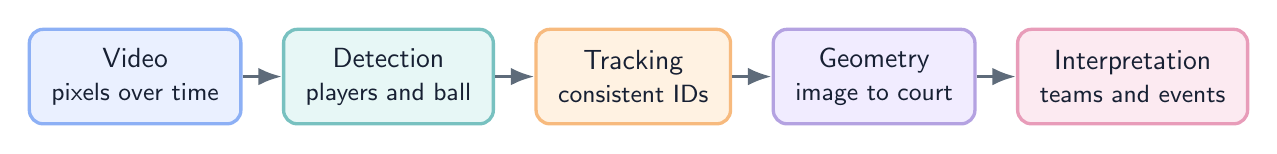
\begin{tikzpicture}[node distance=7mm and 5mm]
\node[flowblue] (video) {Video\\\small pixels over time};
\node[flowteal,right=of video] (det) {Detection\\\small players and ball};
\node[floworange,right=of det] (track) {Tracking\\\small consistent IDs};
\node[flowpurple,right=of track] (geo) {Geometry\\\small image to court};
\node[flowpink,right=of geo] (under) {Interpretation\\\small teams and events};
\draw[arrow] (video)--(det);
\draw[arrow] (det)--(track);
\draw[arrow] (track)--(geo);
\draw[arrow] (geo)--(under);
\end{tikzpicture}
\end{adjustbox}
\end{center}

\begin{plainBox}
\textbf{Errors can occur at every step.}\quad
A missed player detection can interrupt a track. Swapped identities corrupt movement statistics. Inaccurate court calibration makes distance estimates unreliable, and incorrect team labels distort formation and tactical analysis. A usable system must therefore retain intermediate results and confidence information alongside its final output.
\end{plainBox}

\section*{2. Six Core Vision Tasks}

\begin{tcbraster}[raster columns=2,raster equal height=rows,raster column skip=7pt,raster row skip=7pt]
\begin{termBox}{Image classification}
Identifies the main category of an image, such as player, referee or basketball in a cropped image. The output is usually a class label, without an object location.
\end{termBox}
\begin{termBox}{Object detection}
Identifies objects and their locations. Players and balls are commonly represented by bounding boxes. This is a typical first step in video analysis.
\end{termBox}
\begin{termBox}{Image segmentation}
Assigns a label to each pixel. It can describe player outlines, court areas or jerseys more precisely than boxes, but usually requires more annotation work and computation.
\end{termBox}
\begin{termBox}{Keypoints and pose}
Locates points with a defined meaning: court-line intersections or body joints such as shoulders, elbows, wrists and knees. These support angle and movement analysis.
\end{termBox}
\begin{termBox}{Tracking}
Determines whether observations in successive frames belong to the same object. The main task is to maintain identity over time.
\end{termBox}
\begin{termBox}{Action and event understanding}
Identifies events such as a shot release, pass, screen, defensive switch or fast break. It usually combines detection, tracking, pose and temporal signals.
\end{termBox}
\end{tcbraster}

\section*{3. How the Methods Developed}

\begin{historyBox}
\textbf{Stage 1: Rules and traditional image processing.}\quad
Early systems used color thresholds, background subtraction, edges, template matching and optical flow. They could work with fixed cameras and stable lighting, but were sensitive to shadows, occlusion, similar jerseys and camera motion.

\textbf{Stage 2: Handcrafted features and machine learning.}\quad
Researchers combined features such as HOG, SIFT and Haar with classifiers such as SVM and AdaBoost. These generalized better than simple rules, but still depended on manually designed features and had limitations in complex sports scenes.

\textbf{Stage 3: Deep learning for detection.}\quad
The R-CNN family introduced deep features into object detection. Single-stage methods such as SSD and YOLO emphasized real-time performance. Multi-scale features, anchor-free designs and Transformer detectors later improved small-object and crowded-scene detection.

\textbf{Stage 4: Tracking by detection.}\quad
Objects are detected in each frame, then linked using motion models, box overlap and appearance features. SORT, DeepSORT, ByteTrack and BoT-SORT follow this approach, with different association cues and occlusion handling.

\textbf{Stage 5: End-to-end temporal and multimodal analysis.}\quad
More recent methods use Transformers, long-term memory, cross-camera features, language and large vision models. For many practical systems, however, separate detection, tracking and geometry modules remain easier to debug, evaluate and deploy.
\end{historyBox}

\section*{4. Tools and Their Roles}

\begin{toolBox}
\begin{tabularx}{\textwidth}{>{\bfseries\color{Ink}}p{2.7cm} Y Y}
\toprule
Stage & Common tools & Uses and considerations \\
\midrule
Annotation & CVAT, Roboflow Annotate, Label Studio & Create boxes, polygons, masks and keypoints. Consistent rules and version control matter more than the choice of tool.\\
Geometry and image processing & OpenCV, NumPy & Homography, camera calibration, image transforms, optical flow, filtering and visualization.\\
Model training & PyTorch, Ultralytics, MMDetection, Detectron2 & Build detectors. Data formats, licenses and deployment procedures differ between frameworks.\\
Multi-object tracking & ByteTrack, BoT-SORT, DeepSORT, OC-SORT & Link frame-level detections to track IDs. Choose according to camera motion, occlusion and latency requirements.\\
Human pose & MediaPipe, MMPose, OpenPose, RTMPose & Estimate body keypoints. A close-up of one person and distant views of many people pose different challenges.\\
Evaluation and experiments & MOTChallenge tools, COCO metrics, Weights \& Biases, MLflow & Record metrics, failure cases and settings. A few successful demonstrations do not establish overall performance.\\
\bottomrule
\end{tabularx}
\end{toolBox}

\clearpage
\section*{5. The Five-Day Course Plan}

\begin{center}
\begin{adjustbox}{max width=\linewidth}
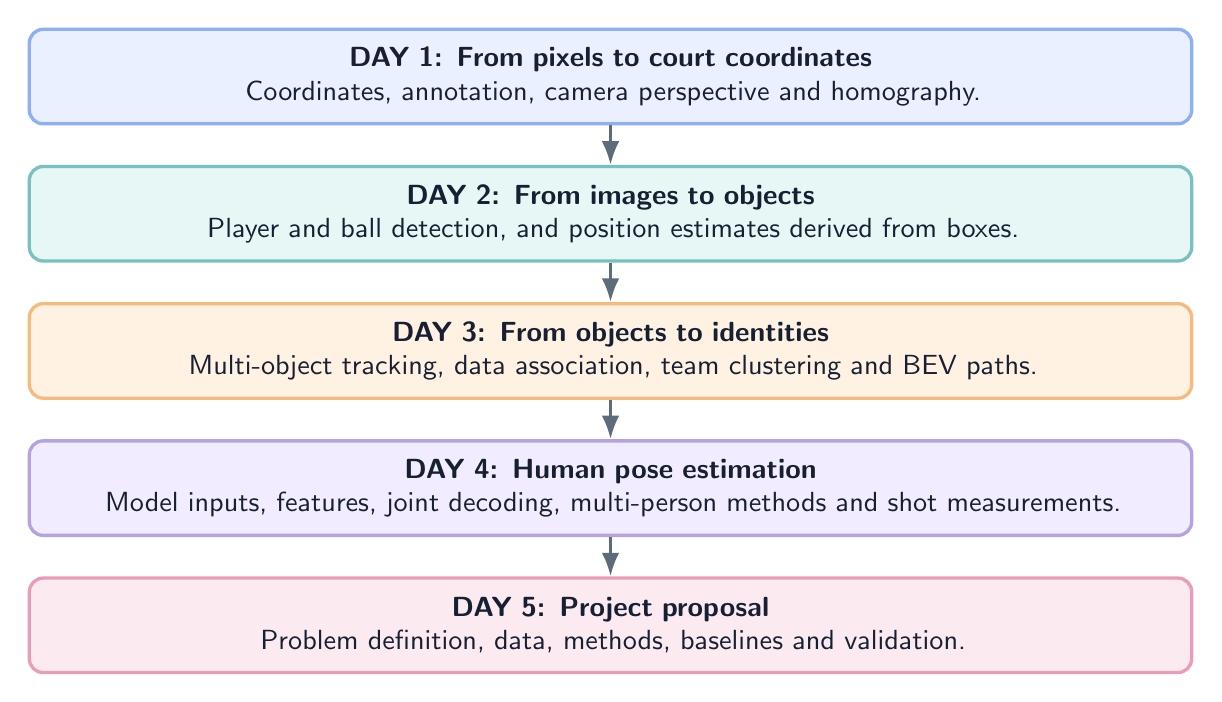
\begin{tikzpicture}[node distance=5mm]
\node[flowblue,text width=14.2cm] (d1) {\textbf{DAY 1: From pixels to court coordinates}\\Coordinates, annotation, camera perspective and homography.};
\node[flowteal,text width=14.2cm,below=of d1] (d2) {\textbf{DAY 2: From images to objects}\\Player and ball detection, and position estimates derived from boxes.};
\node[floworange,text width=14.2cm,below=of d2] (d3) {\textbf{DAY 3: From objects to identities}\\Multi-object tracking, data association, team clustering and BEV paths.};
\node[flowpurple,text width=14.2cm,below=of d3] (d4) {\textbf{DAY 4: Human pose estimation}\\Model inputs, features, joint decoding, multi-person methods and shot measurements.};
\node[flowpink,text width=14.2cm,below=of d4] (d5) {\textbf{DAY 5: Project proposal}\\Problem definition, data, methods, baselines and validation.};
\draw[arrow] (d1)--(d2);\draw[arrow] (d2)--(d3);\draw[arrow] (d3)--(d4);\draw[arrow] (d4)--(d5);
\end{tikzpicture}
\end{adjustbox}
\end{center}

\begin{takeawayBox}
The five days form a connected, inspectable system:
\[
\text{video}\rightarrow\text{detections}\rightarrow\text{tracks}\rightarrow\text{court positions}\rightarrow\text{events}\rightarrow\text{evidence}
\]
Downstream analysis depends on the quality of earlier modules. Each day therefore addresses both the method's capabilities and the conditions under which its output is unreliable.
\end{takeawayBox}

\clearpage
\pagenumbering{arabic}

% ================================================================
% DAY 1
% ================================================================
\chapter{From Image Pixels to the Court: Coordinates, Annotation and Homography}

\begin{heroBox}
\textbf{Main question:}\quad
How can player positions be mapped onto a top-down court diagram when the camera records an oblique, perspective-distorted image?

\textbf{Learning objectives:}\quad
Distinguish image coordinates from court coordinates, select suitable annotations, understand the assumptions and limits of homography, and check the reliability of a projection.
\end{heroBox}

\section{Camera Images Represent Projections}

\begin{conceptBox}
A player moving away from the camera appears smaller without changing height. Parallel sidelines may appear to converge. These changes result from projecting a three-dimensional scene onto an image plane.
\end{conceptBox}

Image coordinates usually start at the top-left corner, with $u$ increasing to the right and $v$ downward, in pixels. Court coordinates can be measured in meters: for example, the lower-left court corner is $(0,0)$, with $X$ along the long side and $Y$ along the short side. These coordinate systems answer different questions.

\begin{itemize}
  \item Image coordinates: Where is the box in the image?
  \item Court coordinates: Where is the player standing on the court?
  \item A bird's-eye view (BEV) provides a shared, top-down coordinate system for comparing distance, speed and positioning.
\end{itemize}

\begin{center}
\begin{adjustbox}{max width=\linewidth}
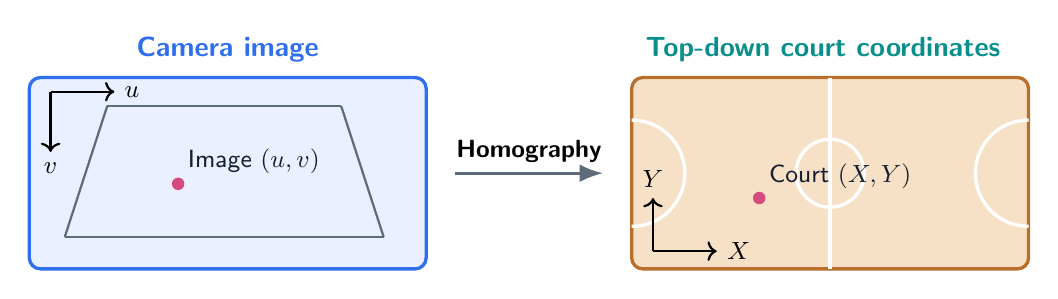
\begin{tikzpicture}[scale=.9]
  % image plane
  \node[font=\bfseries\color{Blue}] at (-4.2,3.1) {Camera image};
  \draw[rounded corners=4pt,fill=BlueSoft,draw=Blue,very thick] (-7,0) rectangle (-1.4,2.7);
  \draw[draw=Muted,thick] (-6.5,.45)--(-2.0,.45);
  \draw[draw=Muted,thick] (-5.9,2.3)--(-2.6,2.3);
  \draw[draw=Muted,thick] (-6.5,.45)--(-5.9,2.3);
  \draw[draw=Muted,thick] (-2.0,.45)--(-2.6,2.3);
  \fill[Pink] (-4.9,1.2) circle (2.5pt) node[above right,text=Ink,font=\small] {Image $(u,v)$};
  \draw[->,thick] (-6.7,2.5)--(-5.8,2.5) node[right,font=\small] {$u$};
  \draw[->,thick] (-6.7,2.5)--(-6.7,1.65) node[below,font=\small] {$v$};
  % arrow
  \draw[arrow] (-1.0,1.35)--(1.1,1.35) node[midway,above,font=\bfseries\small] {Homography};
  % court
  \node[font=\bfseries\color{Teal}] at (4.2,3.1) {Top-down court coordinates};
  \draw[rounded corners=4pt,fill=Court!35,draw=CourtDark,very thick] (1.5,0) rectangle (7.1,2.7);
  \draw[white,line width=1.2pt] (4.3,0)--(4.3,2.7);
  \draw[white,line width=1.2pt] (4.3,1.35) circle (.48);
  \draw[white,line width=1.2pt] (1.5,.6) arc (-90:90:.75);
  \draw[white,line width=1.2pt] (7.1,.6) arc (270:90:.75);
  \fill[Pink] (3.3,1.0) circle (2.5pt) node[above right,text=Ink,font=\small] {Court $(X,Y)$};
  \draw[->,thick] (1.8,.25)--(2.7,.25) node[right,font=\small] {$X$};
  \draw[->,thick] (1.8,.25)--(1.8,1.0) node[above,font=\small] {$Y$};
\end{tikzpicture}
\end{adjustbox}
\end{center}

\section{Choose Annotations to Match the Task}

\subsection{Four Annotation Types and Their Costs}

\begin{tabularx}{\textwidth}{>{\bfseries\RaggedRight}p{2.7cm} Y Y Y}
\toprule
Type & Representation & Suitable questions & Main limitation \\
\midrule
Classification & One label per image & Is this crop a ball, player or referee? & No object location.\\
BBOX & Rectangle $(x_1,y_1,x_2,y_2)$ & Where are players and balls? & Includes background; no precise outline.\\
Segmentation & Pixel-level mask & Jersey regions, player outlines and court areas & Costly annotation and more complex processing.\\
Keypoints & Semantically defined points & Court intersections, joints and rim center & Requires clear visibility rules for occluded points.\\
\bottomrule
\end{tabularx}

\begin{plainBox}
\textbf{Keypoints are commonly used for court calibration.}\quad
Examples include defined intersections of the three-point line and sideline, free-throw line corners, and halfway-line intersections. Their fixed court locations provide image-to-court correspondences.
\end{plainBox}

\subsection{Consistent Rules Matter More Than the Annotation Tool}

Annotators may interpret a player box differently. Should it include shoes or a shadow during a jump? For an occluded player, should it cover the estimated full body or only the visible region? Inconsistent choices introduce \eng{label noise} and give the model contradictory training signals.

Prepare an \eng{annotation guideline} before labeling the full dataset:

\begin{enumerate}
  \item Define every class with positive, negative and borderline examples.
  \item Specify how to handle occlusion, truncation, blur, small objects and objects partly outside the image.
  \item Have several people annotate a small shared sample and review disagreements.
  \item Create a new dataset version whenever rules change; retain previous versions.
  \item Split training, validation and test data by video or game to prevent leakage between adjacent frames.
\end{enumerate}

\begin{riskBox}
\textbf{A common source of data leakage:}\quad
Consecutive frames from the same video are very similar. If frame 100 is used for training and frame 101 for testing, a model may succeed by remembering the scene and jerseys rather than generalizing to a new game.
\end{riskBox}

\section{Homography: Mapping Between Planes}

\subsection{Capabilities and Assumptions}

A homography describes a projective relationship between two planes. In basketball, it commonly maps the court plane in the camera image to a top-down court plane.

In homogeneous coordinates:
\[
\lambda
\begin{bmatrix}X\\Y\\1\end{bmatrix}
=
H
\begin{bmatrix}u\\v\\1\end{bmatrix},
\qquad
H\in\mathbb{R}^{3\times 3}.
\]

$H$ contains nine entries, but multiplying the whole matrix by a nonzero constant leaves the projection unchanged. It therefore has eight degrees of freedom. Each 2D point pair supplies two independent equations, so at least four point pairs in a non-degenerate configuration are required.

\begin{conceptBox}
Think of homography as a way to rectify a perspective view of a flat surface. The mapped points must lie on that plane. A player's head, an airborne ball and the rim are above the floor, so a floor homography cannot map them accurately.
\end{conceptBox}

\subsection{Why Use Homogeneous Coordinates?}

Ordinary 2D matrix multiplication cannot conveniently combine translation with perspective division. Writing a point as $[u,v,1]^\mathsf{T}$ allows translation, rotation, scaling, shear and perspective to be represented by matrix multiplication, followed by division by the third component:
\[
\begin{bmatrix}\tilde X\\\tilde Y\\\tilde W\end{bmatrix}
=H\begin{bmatrix}u\\v\\1\end{bmatrix},
\qquad
X=\frac{\tilde X}{\tilde W},\quad
Y=\frac{\tilde Y}{\tilde W}.
\]

\subsection{DLT, RANSAC and Reprojection Error}

\begin{historyBox}
\textbf{DLT(Direct Linear Transform)}\quad
Rewrites point correspondences as homogeneous linear equations and solves them using SVD. It is fast and often supplies an initial estimate, but is sensitive to incorrect correspondences.

\textbf{RANSAC}\quad
Repeatedly fits a model to a minimal random sample and counts supporting observations. Its main purpose is to identify outliers rather than force the model to fit every point.
\end{historyBox}

Reprojection error is defined as:
\[
e_i=\left\|\widehat{\mathbf q}_i-\mathbf q_i\right\|_2,
\qquad
\widehat{\mathbf q}_i=\pi(H\mathbf p_i),
\]
Here, $\pi(\cdot)$ divides by the homogeneous scale. Review the maximum error, error distribution and spatial pattern as well as the mean.

\begin{pseudoBox}
INPUT: camera keypoints P, matching court points Q

REPEAT many trials
  randomly sample at least four non-collinear pairs
  estimate a candidate homography H
  project every camera point through H
  compute reprojection errors
  mark small-error pairs as inliers
KEEP the candidate with the strongest inlier support
REFIT H using all inliers
VALIDATE on independent court points, not only training pairs
\end{pseudoBox}

\subsection{Selecting and Checking Calibration Points}

\begin{itemize}
  \item Spread points across the visible court rather than concentrating them near the image center.
  \item Avoid nearly collinear configurations, which cannot stably constrain a full planar transform.
  \item Prefer sharp line intersections with an unambiguous definition.
  \item Do not treat an indistinct point on the three-point arc as an exact intersection without a clear geometric definition.
  \item Use validation points that were not used to estimate $H$.
\end{itemize}

\begin{center}
\begin{adjustbox}{max width=\linewidth}
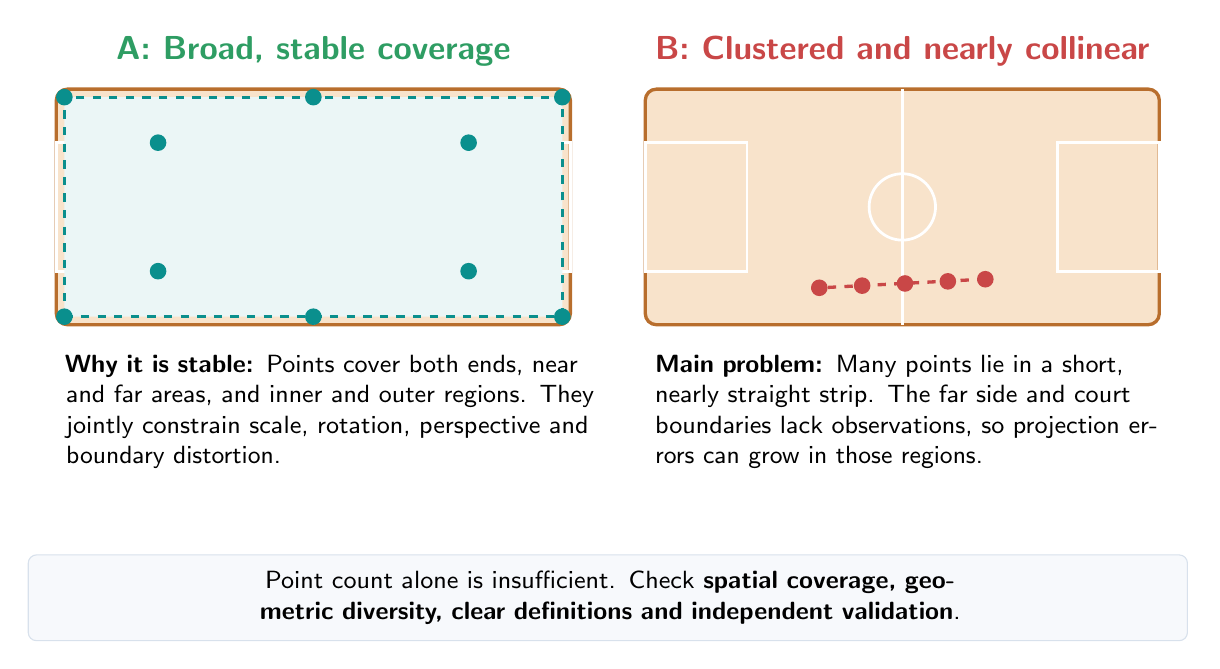
\begin{tikzpicture}[x=.68cm,y=.68cm,font=\small]
\begin{scope}[shift={(0,0)}]
  \node[font=\bfseries\large,text=Green] at (4.8,6.2) {A: Broad, stable coverage};
  \draw[rounded corners=4pt,fill=Court!32,draw=CourtDark,very thick] (0,1.1) rectangle (9.6,5.5);
  \draw[white,line width=1.0pt] (4.8,1.1)--(4.8,5.5);
  \draw[white,line width=1.0pt] (4.8,3.3) circle (.62);
  \draw[white,line width=1.0pt] (0,2.1) rectangle (1.9,4.5);
  \draw[white,line width=1.0pt] (9.6,2.1) rectangle (7.7,4.5);
  \draw[Teal,dashed,line width=1.2pt,fill=Teal!8]
    (.15,1.25)--(4.8,1.25)--(9.45,1.25)--(9.45,5.35)--(4.8,5.35)--(.15,5.35)--cycle;
  \foreach \p in {(.15,1.25),(.15,5.35),(9.45,1.25),(9.45,5.35),(4.8,1.25),(4.8,5.35),(1.9,2.1),(1.9,4.5),(7.7,2.1),(7.7,4.5)}
    \fill[Teal] \p circle (3.0pt);
  \node[align=left,text width=6.7cm,anchor=north west] at (0,.72)
    {\textbf{Why it is stable:} Points cover both ends, near and far areas, and inner and outer regions. They jointly constrain scale, rotation, perspective and boundary distortion.};
\end{scope}
\begin{scope}[shift={(11.0,0)}]
  \node[font=\bfseries\large,text=Red] at (4.8,6.2) {B: Clustered and nearly collinear};
  \draw[rounded corners=4pt,fill=Court!32,draw=CourtDark,very thick] (0,1.1) rectangle (9.6,5.5);
  \draw[white,line width=1.0pt] (4.8,1.1)--(4.8,5.5);
  \draw[white,line width=1.0pt] (4.8,3.3) circle (.62);
  \draw[white,line width=1.0pt] (0,2.1) rectangle (1.9,4.5);
  \draw[white,line width=1.0pt] (9.6,2.1) rectangle (7.7,4.5);
  \draw[Red,dashed,line width=1.2pt] (3.1,1.78)--(6.5,1.96);
  \foreach \p in {(3.25,1.79),(4.05,1.83),(4.85,1.87),(5.65,1.91),(6.35,1.95)}
    \fill[Red] \p circle (3.0pt);
  \node[align=left,text width=6.7cm,anchor=north west] at (0,.72)
    {\textbf{Main problem:} Many points lie in a short, nearly straight strip. The far side and court boundaries lack observations, so projection errors can grow in those regions.};
\end{scope}
\node[draw=Line,fill=Paper,rounded corners=3pt,inner sep=6pt,text width=14.3cm,align=center] at (10.3,-4.0)
  {Point count alone is insufficient. Check \textbf{spatial coverage, geometric diversity, clear definitions and independent validation}.};
\end{tikzpicture}
\end{adjustbox}
\end{center}

\section{From Boxes to Court Positions: The Footpoint Approximation}

A player box covers the whole body, whereas homography assumes a point on the floor. The bottom-center of the box is often used as a footpoint because it approximates the location of the shoes:
\[
\mathbf f=\left(\frac{x_1+x_2}{2},\;y_2\right).
\]

\begin{center}
\begin{adjustbox}{max width=\linewidth}
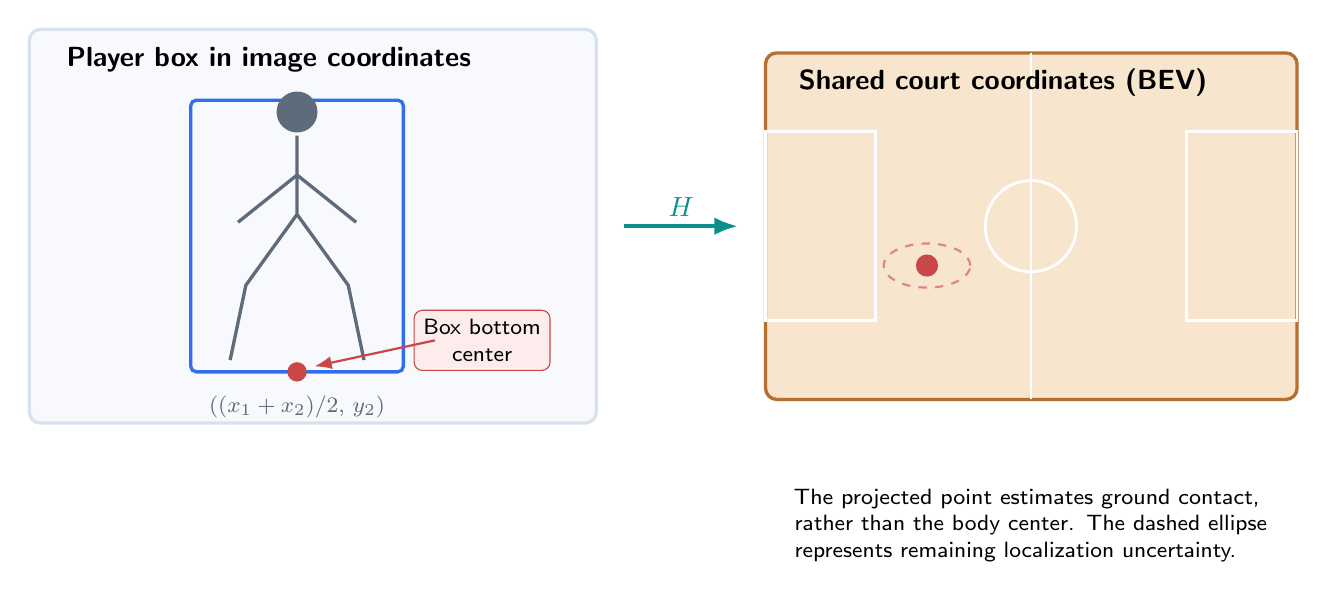
\begin{tikzpicture}[x=1cm,y=1cm,font=\footnotesize]
  \draw[rounded corners=4pt,fill=Paper,draw=Line,very thick] (0,0) rectangle (7.2,5.0);
  \node[anchor=west,font=\bfseries] at (.35,4.62) {Player box in image coordinates};
  \draw[Blue,very thick,rounded corners=2pt] (2.05,.65) rectangle (4.75,4.1);
  \draw[Muted,very thick] (3.4,3.65)--(3.4,2.65)--(2.75,1.75)--(2.55,.8);
  \draw[Muted,very thick] (3.4,2.65)--(4.05,1.75)--(4.25,.8);
  \draw[Muted,very thick] (3.4,3.15)--(2.65,2.55);
  \draw[Muted,very thick] (3.4,3.15)--(4.15,2.55);
  \fill[Muted] (3.4,3.95) circle (.26);
  \fill[Red] (3.4,.65) circle (3.5pt);
  \node[fill=RedSoft,draw=Red,rounded corners=3pt,align=center] at (5.75,1.05) {Box bottom\\center};
  \draw[thinArrow,Red] (5.15,1.05)--(3.62,.72);
  \node[text=Muted] at (3.4,.20) {$((x_1+x_2)/2,\,y_2)$};
  \draw[-{Latex[length=3mm]},line width=1.4pt,draw=Teal] (7.55,2.5)--(9.0,2.5);
  \node[above,text=Teal,font=\bfseries] at (8.28,2.5) {$H$};
  \draw[rounded corners=4pt,fill=Court!30,draw=CourtDark,very thick] (9.35,.3) rectangle (16.1,4.7);
  \draw[white,line width=1pt] (12.72,.3)--(12.72,4.7);
  \draw[white,line width=1pt] (12.72,2.5) circle (.58);
  \draw[white,line width=1pt] (9.35,1.3) rectangle (10.75,3.7);
  \draw[white,line width=1pt] (16.1,1.3) rectangle (14.7,3.7);
  \fill[Red] (11.4,2.0) circle (4pt);
  \draw[Red!65,dashed,thick] (11.4,2.0) ellipse (.55 and .28);
  \node[anchor=west,font=\bfseries] at (9.65,4.32) {Shared court coordinates (BEV)};
  \node[align=left,text width=6.0cm,fill=white,rounded corners=3pt,inner sep=4pt] at (12.72,-1.3)
    {The projected point estimates ground contact, rather than the body center. The dashed ellipse represents remaining localization uncertainty.};
\end{tikzpicture}
\end{adjustbox}
\end{center}

This approximation can fail when:

\begin{itemize}
  \item The player jumps and both shoes leave the floor.
  \item The box excludes the feet or another player occludes them.
  \item The player is lying or sitting down, or only the upper body is visible.
  \item A strongly oblique view makes the box's bottom-center differ from the actual foot-contact position.
\end{itemize}

Ankle keypoints, shoe segmentation or temporal footpoint smoothing may improve estimates. Greater complexity does not guarantee greater accuracy; validate against known court positions.


\section{Tools and Practical Workflow}


\begin{toolBox}
\textbf{OpenCV:}\quad
\texttt{findHomography}, \texttt{perspectiveTransform} and \texttt{warpPerspective} provide standard numerical operations. They do not check whether the selected points are appropriate.

\textbf{Roboflow / CVAT / Label Studio:}\quad
Support keypoints, boxes, polygons and dataset versions. Annotation guidelines, quality checks and split design still require careful planning.

\textbf{NumPy / Pandas:}\quad
Useful for storing point correspondences, computing errors, exporting CSV files and building reproducible processing workflows.
\end{toolBox}

\section{Day 1 Review Checklist}

\begin{takeawayBox}
\begin{itemize}
  \item Are image pixels, BEV pixels and physical meters clearly distinguished?
  \item Are calibration points well distributed, non-degenerate and consistently defined?
  \item Are independent validation points available?
  \item Is ground contact distinguished from the body center?
  \item Is the planar method being incorrectly applied to an airborne ball or upper-body point?
\end{itemize}
\end{takeawayBox}

\begin{questionBox}
Why can a box that looks accurate in the image produce a large BEV error? Discuss box localization, the footpoint approximation, homography and perspective amplification.
\end{questionBox}

% ================================================================
% DAY 2
% ================================================================
\chapter{Finding Players and Balls: Object Detection and BBOX-to-BEV}

\begin{heroBox}
\textbf{Main question:}\quad
How does a model turn millions of pixels into player and ball detections? What do its confidence scores, boxes and class labels mean?
\end{heroBox}

\section{Why Classification Alone Is Insufficient}

\begin{conceptBox}
An image classifier can indicate that a basketball is present but cannot locate it. A game frame contains several players, referees and a ball, so object detection must return multiple locations and class labels.
\end{conceptBox}

A detection commonly contains:
\[
D_i=(x_1,y_1,x_2,y_2,\;c,\;s),
\]
Here, $(x_1,y_1,x_2,y_2)$ defines the box, $c$ is the class and $s$ is the model score. The score is usually a confidence measure for ranking and filtering, rather than a statistically calibrated probability of correctness.

\section{From Sliding Windows to End-to-End Detection}

\begin{historyBox}
\textbf{Sliding windows and handcrafted features:}\quad
Windows of different sizes are moved across the image. Features such as HOG or Haar are computed for each window and passed to a classifier. This requires many candidate windows and considerable manual feature design.

\textbf{Two-stage detector:}\quad
R-CNN, Fast R-CNN and Faster R-CNN first propose regions that may contain objects, then classify them and refine their boxes. They can be accurate, but use a more involved processing pipeline.

\textbf{One-stage detector:}\quad
SSD and YOLO treat detection as dense prediction. One forward pass produces many candidate boxes, making them suitable for real-time video.

\textbf{Anchor-free and Transformer detectors:}\quad
Later designs reduce manual anchor design or use set prediction and attention. They change candidate generation and matching, but still face small balls, occlusion and dataset bias.
\end{historyBox}

\section{Three Main Components of a Modern Detector}

\begin{center}
\begin{adjustbox}{max width=\linewidth}
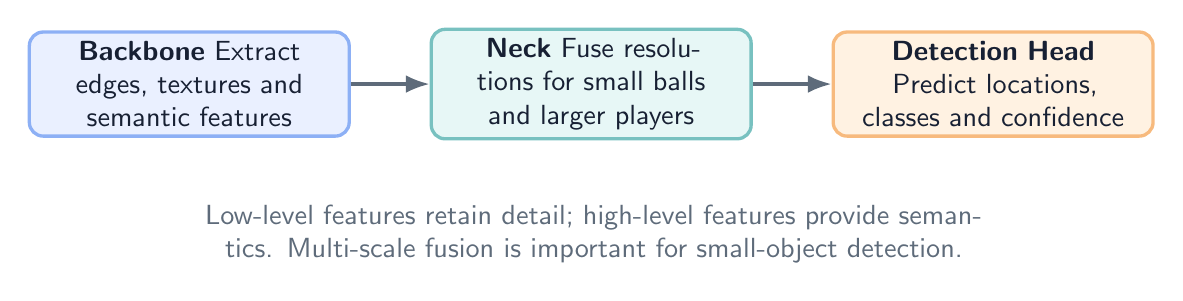
\begin{tikzpicture}[node distance=10mm]
\node[flowblue,text width=3.5cm] (back) {\textbf{Backbone}\
Extract edges, textures and semantic features};
\node[flowteal,text width=3.5cm,right=of back] (neck) {\textbf{Neck}\
Fuse resolutions for small balls and larger players};
\node[floworange,text width=3.5cm,right=of neck] (head) {\textbf{Detection Head}\
Predict locations, classes and confidence};
\draw[arrow] (back)--(neck);\draw[arrow] (neck)--(head);
\node[below=7mm of neck,text=Muted,text width=12cm,align=center] {Low-level features retain detail; high-level features provide semantics. Multi-scale fusion is important for small-object detection.};
\end{tikzpicture}
\end{adjustbox}
\end{center}

\subsection{Why Is the Ball Harder to Detect Than a Player?}

\begin{itemize}
  \item A distant ball may occupy only a dozen pixels, or fewer.
  \item Fast motion blurs the ball's boundary.
  \item Hands, bodies and the rim often occlude the ball.
  \item Lighting, rotation and video compression alter its appearance.
  \item Background locations greatly outnumber ball locations, creating class and scale imbalance.
\end{itemize}

Possible improvements include higher input resolution, more distant-ball examples, cropping or tiling, revised augmentation, high-resolution feature layers, temporal tracking and a dedicated ball detector.

\section{Confidence, Precision and Recall}

\subsection{The Confidence Threshold Controls a Trade-off}

Lowering the confidence threshold retains more candidates, reducing missed objects but increasing false positives. Raising it usually has the opposite effect.

\[
\mathrm{Precision}=\frac{TP}{TP+FP},
\qquad
\mathrm{Recall}=\frac{TP}{TP+FN}.
\]

\begin{center}
\begin{adjustbox}{max width=\linewidth}
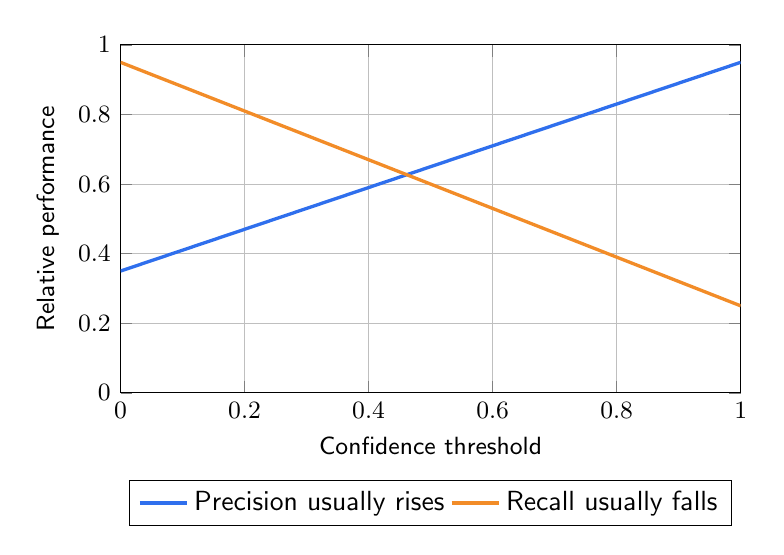
\begin{tikzpicture}
\begin{axis}[
width=.78\textwidth,height=6cm,
xlabel={Confidence threshold},ylabel={Relative performance},xmin=0,xmax=1,ymin=0,ymax=1,
grid=both,legend style={at={(.5,-.25)},anchor=north,legend columns=2},
tick label style={font=\small},label style={font=\small}]
\addplot[very thick,Blue,domain=0:1,samples=100] {0.35+0.6*x};
\addlegendentry{Precision usually rises}
\addplot[very thick,Orange,domain=0:1,samples=100] {0.95-0.7*x};
\addlegendentry{Recall usually falls}
\end{axis}
\end{tikzpicture}
\end{adjustbox}
\end{center}

The figure is conceptual; actual curves need not be linear. Choose thresholds on the validation set according to application costs. Ball tracking may benefit from retaining low-score true-ball candidates and rejecting background through temporal association.

\subsection{IoU: Measuring Box Overlap}

Intersection over Union:
\[
\mathrm{IoU}(A,B)=\frac{|A\cap B|}{|A\cup B|}.
\]

IoU is used to compare predictions with ground truth, suppress duplicates in NMS and associate detections with tracks. These uses require separate thresholds with different meanings.

\section{NMS: Removing Duplicate Detections}

Dense detectors often produce several candidates around one object. Non-maximum suppression (NMS) ranks them by score, keeps the highest-scoring box and removes boxes that overlap it too strongly.

\begin{pseudoBox}
SORT all candidate boxes by confidence
WHILE candidates remain
  take the highest-score box as a kept detection
  compare it with the remaining boxes
  suppress boxes whose IoU is above the NMS threshold
RETURN all kept detections
\end{pseudoBox}

\begin{riskBox}
Two players near the basket may have heavily overlapping boxes. An NMS threshold that is too low can remove a real player; one that is too high can leave duplicates. The threshold balances duplicate removal against retaining nearby objects.
\end{riskBox}

\section{From Detection to BEV: Data Flow and Error Sources}

\begin{center}
\begin{adjustbox}{max width=\linewidth}
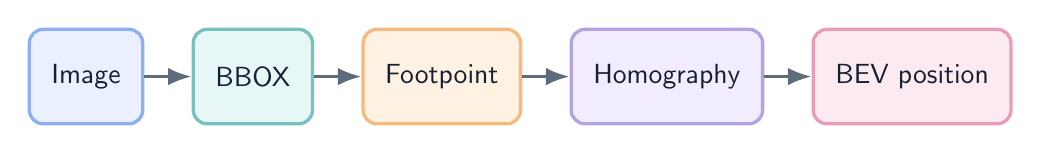
\begin{tikzpicture}[node distance=6mm]
\node[flowblue] (img) {Image};
\node[flowteal,right=of img] (bbox) {BBOX};
\node[floworange,right=of bbox] (foot) {Footpoint};
\node[flowpurple,right=of foot] (h) {Homography};
\node[flowpink,right=of h] (bev) {BEV position};
\draw[arrow] (img)--(bbox);\draw[arrow] (bbox)--(foot);\draw[arrow] (foot)--(h);\draw[arrow] (h)--(bev);
\end{tikzpicture}
\end{adjustbox}
\end{center}

The final position can be written as:
\[
\mathbf q=g(H,\mathbf f(B)).
\]
At least three sources contribute to its error:

\begin{enumerate}
  \item Localization error in the detected box.
  \item Approximation error when deriving the footpoint from the box.
  \item Homography estimation error and spatial extrapolation error.
\end{enumerate}

\begin{plainBox}
\textbf{Evaluate the components separately.}\quad
Final BEV error alone cannot distinguish detection problems from geometry problems. Likewise, mAP alone cannot establish court-position accuracy. Record box metrics, footpoint pixel error, homography validation error and final position error in meters.
\end{plainBox}

\section{Tools and Suitable Uses}

\begin{toolBox}
\begin{itemize}
  \item \textbf{Ultralytics YOLO:} A concise API for training, inference and tracking integration. Check versions, model licenses and defaults.
  \item \textbf{MMDetection:} Extensive research configurations for comparing detectors and losses, with a steeper learning curve.
  \item \textbf{Detectron2:} Suitable for research and customization with Faster R-CNN, Mask R-CNN and related methods.
  \item \textbf{TensorRT / ONNX Runtime:} Support deployment and acceleration; they do not inherently improve recognition accuracy.
  \item \textbf{Roboflow:} Supports data management, format conversion, training and deployment. Dataset quality still requires direct review.
\end{itemize}
\end{toolBox}

\section{Interpreting and Evaluating Detections}

\begin{takeawayBox}
\begin{itemize}
  \item Class, location and confidence are distinct outputs.
  \item Confidence is not a guaranteed accuracy rate. Set thresholds using validation data and application costs.
  \item For a small ball, appropriate data scale and temporal information often matter more than a larger model.
  \item NMS and tracking association are separate stages; their IoU thresholds have different roles.
  \item Frame-level detections have no persistent identity and do not constitute tracking.
\end{itemize}
\end{takeawayBox}

% ================================================================
% DAY 3
% ================================================================
\chapter{Maintaining Identities and Teams: Multi-Object Tracking}

\begin{heroBox}
\textbf{Main question:}\quad
With a dozen or more boxes in each frame, how does the system identify the box belonging to the same player in the next frame? Can it restore that identity after occlusion?
\end{heroBox}

\section{Tracking Means Maintaining Identity}

\begin{conceptBox}
Detection finds objects independently in each image. Tracking links observations over time. Even perfect detections cannot identify a player's path if the box order changes between frames.
\end{conceptBox}

A typical multi-object tracking (MOT) output is:
\[
(t,\mathrm{track\_id},x_1,y_1,x_2,y_2,\mathrm{class},\mathrm{score}).
\]

A track ID is a temporary identifier within a video. It is not a jersey number or a player's name. Mapping it to a real player usually requires jersey OCR, ReID, rosters and manual correction.

\section{From Optical Flow to Data Association}

\begin{historyBox}
\textbf{Template matching / Optical Flow:}\quad
Follow the movement of image texture from the preceding frame. Useful for short local tracks, but susceptible to drift with appearance changes, occlusion and large displacement.

\textbf{Kalman Filter + Assignment:}\quad
Predict the next location with a motion model, then match detections to tracks. SORT is a representative lightweight method.

\textbf{Appearance / ReID:}\quad
DeepSORT adds appearance embeddings, comparing player crops as well as positions to help maintain identity after occlusion.

\textbf{Using low-score detections:}\quad
ByteTrack uses some low-score boxes to recover existing tracks affected by blur or occlusion, rather than discarding them all.

\textbf{Camera motion and multiple cues:}\quad
BoT-SORT adds camera-motion compensation and optional ReID. OC-SORT improves observation-based correction for nonlinear motion and occlusion.

\textbf{Transformer / Memory-based MOT:}\quad
Newer methods use attention and memory to model longer-term relationships directly, usually with greater computational cost, data requirements and deployment complexity.
\end{historyBox}

\section{The Tracking-by-Detection Pipeline}

\begin{center}
\begin{adjustbox}{max width=\linewidth}
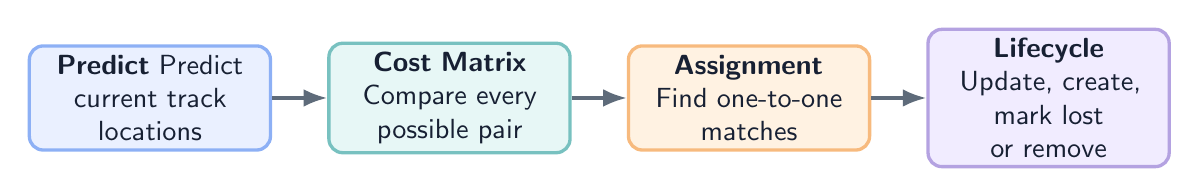
\begin{tikzpicture}[node distance=7mm]
\node[flowblue,text width=2.5cm] (pred) {\textbf{Predict}\
Predict current track locations};
\node[flowteal,text width=2.5cm,right=of pred] (cost) {\textbf{Cost Matrix}\
Compare every possible pair};
\node[floworange,text width=2.5cm,right=of cost] (assign) {\textbf{Assignment}\
Find one-to-one matches};
\node[flowpurple,text width=2.5cm,right=of assign] (life) {\textbf{Lifecycle}\
Update, create, mark lost or remove};
\draw[arrow] (pred)--(cost);\draw[arrow] (cost)--(assign);\draw[arrow] (assign)--(life);
\end{tikzpicture}
\end{adjustbox}
\end{center}

\subsection{Motion Models: Predicting the Next Location}

A Kalman filter commonly represents position, scale and velocity as a state. It predicts the next state from previous frames and corrects it with detections. It estimates motion under noise assumptions; it does not recognize a person's identity.

Sudden stops, turns, jumps, screens and camera motion violate a simple constant-velocity model. Prediction narrows the search region but cannot guarantee identity by itself.

\subsection{The Cost Matrix: Comparing Candidate Matches}

For $m$ existing tracks and $n$ current detections, a cost matrix can be defined as:
\[
C\in\mathbb{R}^{m\times n},
\qquad
C_{ij}=1-\mathrm{IoU}(T_i,D_j)
\]
Alternatively, combine several cues:
\[
C_{ij}=\alpha C^{\mathrm{motion}}_{ij}
+\beta C^{\mathrm{IoU}}_{ij}
+\gamma C^{\mathrm{appearance}}_{ij}.
\]

\begin{center}
\begin{adjustbox}{max width=\linewidth}
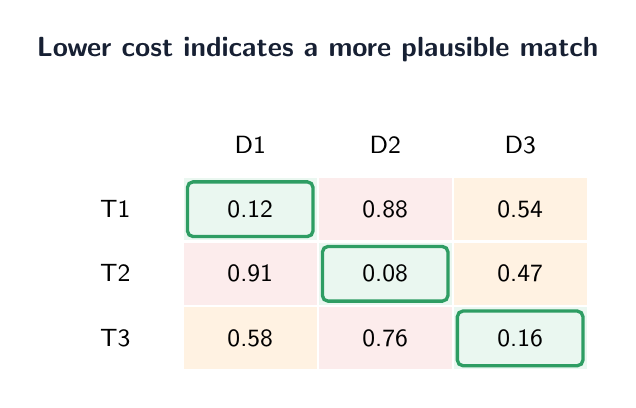
\begin{tikzpicture}
\matrix[matrix of nodes,nodes={minimum width=1.7cm,minimum height=.8cm,draw=white,font=\small},column sep=0pt,row sep=0pt] (m) {
 & D1 & D2 & D3 \\
T1 & |[fill=GreenSoft]| 0.12 & |[fill=RedSoft]| 0.88 & |[fill=OrangeSoft]| 0.54 \\
T2 & |[fill=RedSoft]| 0.91 & |[fill=GreenSoft]| 0.08 & |[fill=OrangeSoft]| 0.47 \\
T3 & |[fill=OrangeSoft]| 0.58 & |[fill=RedSoft]| 0.76 & |[fill=GreenSoft]| 0.16 \\
};
\node[above=4mm of m,font=\bfseries\color{Ink}] {Lower cost indicates a more plausible match};
\draw[Green,very thick,rounded corners=2pt] ($(m-2-2.north west)+(.06,-.06)$) rectangle ($(m-2-2.south east)+(-.06,.06)$);
\draw[Green,very thick,rounded corners=2pt] ($(m-3-3.north west)+(.06,-.06)$) rectangle ($(m-3-3.south east)+(-.06,.06)$);
\draw[Green,very thick,rounded corners=2pt] ($(m-4-4.north west)+(.06,-.06)$) rectangle ($(m-4-4.south east)+(-.06,.06)$);
\end{tikzpicture}
\end{adjustbox}
\end{center}

\subsection{Hungarian Assignment: Optimizing the Overall Match}

Greedy matching repeatedly selects the lowest current cost. It is fast, but an early choice may block a better overall assignment. The Hungarian algorithm minimizes total cost under one-to-one constraints.

Gating is still necessary: reject pairs with excessive distance, insufficient IoU or incompatible appearance instead of forcing a match.

\section{ByteTrack: The Value of Low-Score Boxes}

Discarding all low-confidence detections before tracking can remove real players who are blurred, occluded or only partly visible, breaking their tracks.

ByteTrack uses two association stages:

\begin{plainBox}
\begin{enumerate}[label=\textbf{Step \arabic*:},leftmargin=4.8em,itemsep=.35em]
  \item Divide detections into high- and low-score groups.
  \item Predict where existing tracks should appear in the current frame.
  \item Match high-score boxes first to obtain reliable updates and identify unmatched tracks.
  \item Match remaining tracks to low-score boxes to recover weak observations caused by occlusion or blur.
  \item Create new tracks only from eligible unmatched high-score boxes. Low-score boxes generally do not create new identities on their own.
  \item Retain temporarily unmatched tracks in a lost buffer and remove them after the retention period expires.
\end{enumerate}
\end{plainBox}

\begin{center}
\begin{adjustbox}{max width=\linewidth}
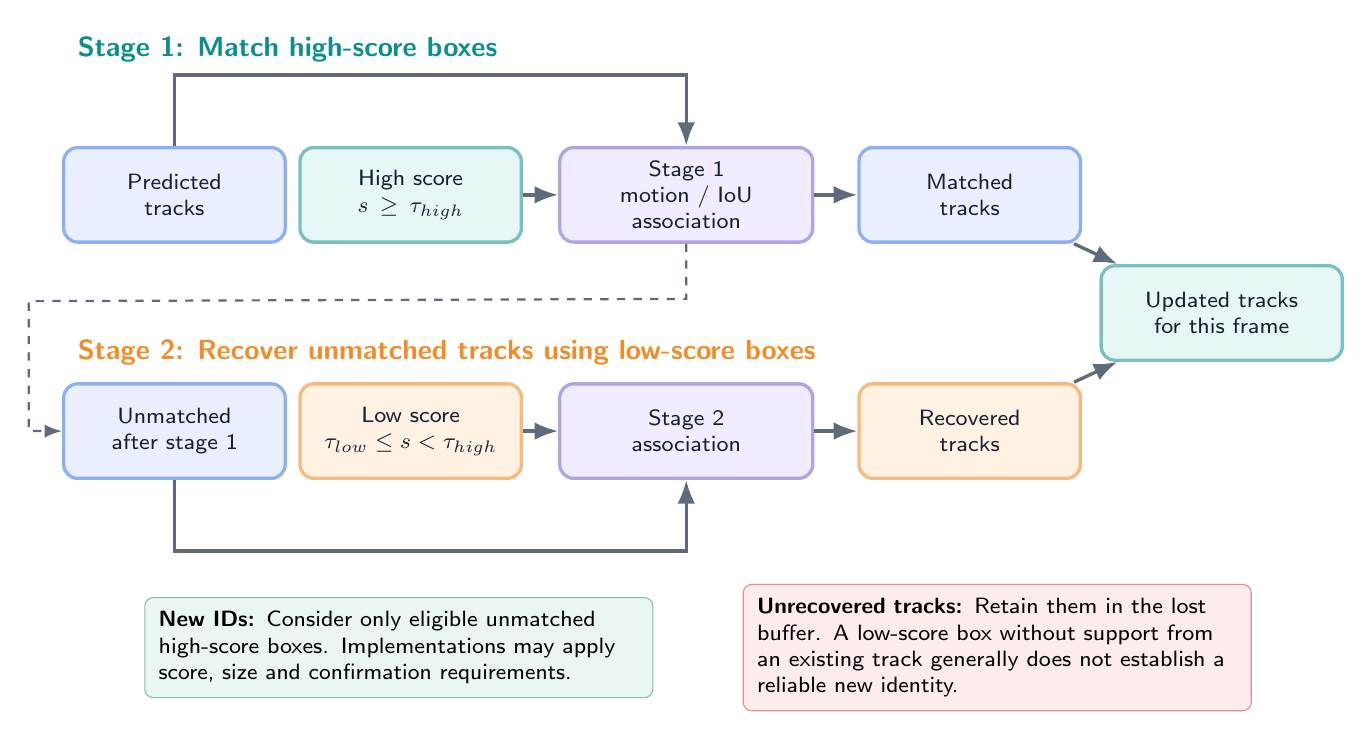
\begin{tikzpicture}[x=1cm,y=1cm,font=\footnotesize]
  \node[font=\bfseries,text=Teal,anchor=west] at (0,5.0) {Stage 1: Match high-score boxes};
  \node[font=\bfseries,text=Orange,anchor=west] at (0,1.15) {Stage 2: Recover unmatched tracks using low-score boxes};
  \node[flowblue,text width=2.25cm] (pred) at (1.35,3.15) {Predicted\\tracks};
  \node[flowteal,text width=2.25cm] (high) at (4.35,3.15) {High score\\$s \geq \tau_{high}$};
  \node[flowpurple,text width=2.65cm] (match1) at (7.85,3.15) {Stage 1\\motion / IoU\\association};
  \node[flowblue,text width=2.25cm] (matched) at (11.45,3.15) {Matched\\tracks};
  \node[flowblue,text width=2.25cm] (unmatched) at (1.35,.15) {Unmatched\\after stage 1};
  \node[floworange,text width=2.25cm] (low) at (4.35,.15) {Low score\\$\tau_{low}\leq s<\tau_{high}$};
  \node[flowpurple,text width=2.65cm] (match2) at (7.85,.15) {Stage 2\\association};
  \node[floworange,text width=2.25cm] (recovered) at (11.45,.15) {Recovered\\tracks};
  \node[flowteal,text width=2.5cm] (out) at (14.65,1.65) {Updated tracks\\for this frame};
  \draw[arrow] (pred.north) -- ++(0,.9) -| (match1.north); \draw[arrow] (high)--(match1); \draw[arrow] (match1)--(matched); \draw[arrow] (matched)--(out);
  \draw[arrow] (unmatched.south) -- ++(0,-.9) -| (match2.south); \draw[arrow] (low)--(match2); \draw[arrow] (match2)--(recovered); \draw[arrow] (recovered)--(out);
  \draw[thinArrow,dashed] (match1.south) -- ++(0,-.7) -- (-.5,1.8) |- (unmatched.west);
  \node[draw=Green!60,fill=GreenSoft,rounded corners=3pt,text width=6.1cm,align=left,inner sep=5pt] at (4.2,-2.6)
    {\textbf{New IDs:} Consider only eligible unmatched high-score boxes. Implementations may apply score, size and confirmation requirements.};
  \node[draw=Red!60,fill=RedSoft,rounded corners=3pt,text width=6.1cm,align=left,inner sep=5pt] at (11.8,-2.6)
    {\textbf{Unrecovered tracks:} Retain them in the lost buffer. A low-score box without support from an existing track generally does not establish a reliable new identity.};
\end{tikzpicture}
\end{adjustbox}
\end{center}

\begin{plainBox}
\textbf{Example:} An attacker moves behind a screener and is only partly visible for several frames. Confidence may fall from 0.86 to 0.28 while the box still overlaps the predicted track location. Stage 2 can retain the original ID. A new 0.28-score box in a corner of the image should not immediately become a new player.
\end{plainBox}

\section{The Track Lifecycle}

A single detection does not immediately establish a reliable identity, and one missed frame need not end a track. Lifecycle management accumulates evidence, tolerates brief occlusion and prevents unsupported tracks from persisting indefinitely.

\begin{center}
\begin{adjustbox}{max width=\linewidth}
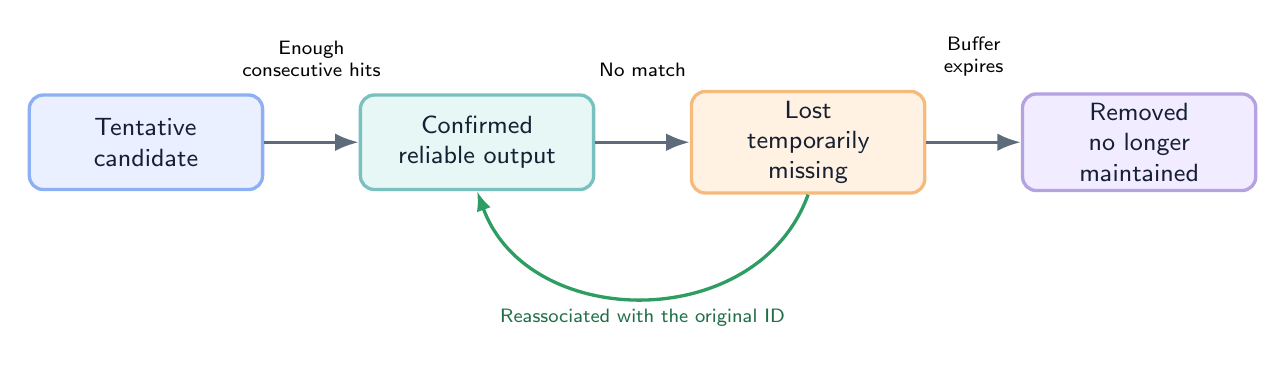
\begin{tikzpicture}[node distance=12mm,font=\small]
  \node[flowblue,text width=2.4cm] (tent) {Tentative\\candidate};
  \node[flowteal,text width=2.4cm,right=of tent] (conf) {Confirmed\\reliable output};
  \node[floworange,text width=2.4cm,right=of conf] (lost) {Lost\\temporarily missing};
  \node[flowpurple,text width=2.4cm,right=of lost] (rem) {Removed\\no longer maintained};
  \draw[arrow] (tent)--(conf) node[midway,above=7mm,text width=2cm,align=center,font=\scriptsize,align=center] {Enough\\consecutive hits};
  \draw[arrow] (conf)--(lost) node[midway,above=7mm,text width=2cm,align=center,font=\scriptsize] {No match};
  \draw[arrow] (lost)--(rem) node[midway,above=7mm,text width=2cm,align=center,font=\scriptsize,align=center] {Buffer\\expires};
  \draw[-{Latex[length=2.5mm]},very thick,draw=Green] (lost.south) to[out=250,in=290,looseness=1.15]
    node[below,font=\scriptsize,text=Green!70!black] {Reassociated with the original ID} (conf.south);
\end{tikzpicture}
\end{adjustbox}
\end{center}

\Needspace{10\baselineskip}
Common states:

\begin{tabularx}{\textwidth}{>{\bfseries\RaggedRight}p{2.6cm} Y Y}
\toprule
State & Meaning & Purpose \\
\midrule
Tentative & Newly created; insufficient evidence & Prevent a one-frame false positive from becoming a stable track.\\
Active / Confirmed & Repeatedly supported by detections & Suitable for output and analysis.\\
Lost & Temporarily unmatched but retained & Tolerate short occlusions and missed detections.\\
Removed & Retention period has expired & Release obsolete state.\\
\bottomrule
\end{tabularx}

\begin{riskBox}
\textbf{Buffer too short:} Brief occlusion produces a new ID.\quad
\textbf{Buffer too long:} An old track may attach to another player.\quad
Set parameters according to FPS, occlusion duration and player density rather than copying defaults.
\end{riskBox}

\section{ReID and Team Recognition: Adding Appearance}

\subsection{What Is Re-identification?}

ReID converts player crops into embeddings, ideally placing the same person's features closer together than different people's features. It can help after long occlusion, but basketball presents similar jerseys, small numbers, changing poses and large front-to-back appearance differences.

ReID is generally an appearance cue for association, not facial recognition.

\subsection{Team Clustering Without Labels}

A simple approach crops the torso, extracts an HSV histogram and uses K-means to form two clusters:
\[
\min_{\{c_i\},\{\boldsymbol\mu_k\}}
\sum_i\left\|\mathbf x_i-\boldsymbol\mu_{c_i}\right\|_2^2.
\]

\begin{center}
\begin{adjustbox}{max width=\linewidth}
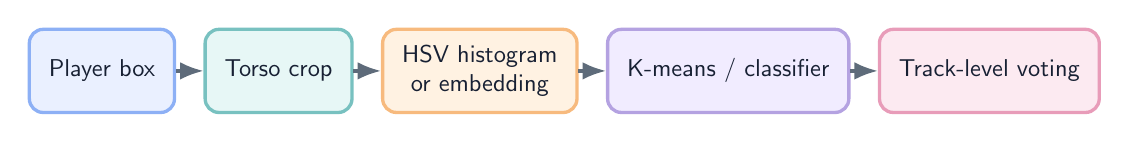
\begin{tikzpicture}[node distance=4mm,scale=.88,transform shape]
\node[flowblue] (crop) {Player box};
\node[flowteal,right=of crop] (torso) {Torso crop};
\node[floworange,right=of torso] (feat) {HSV histogram\\or embedding};
\node[flowpurple,right=of feat] (cluster) {K-means / classifier};
\node[flowpink,right=of cluster] (vote) {Track-level voting};
\draw[arrow] (crop)--(torso);\draw[arrow] (torso)--(feat);\draw[arrow] (feat)--(cluster);\draw[arrow] (cluster)--(vote);
\end{tikzpicture}
\end{adjustbox}
\end{center}

Single-frame clustering is sensitive to occlusion, shadows and background. Collecting features across a track and averaging or voting is usually more reliable. With known team labels, a supervised classifier is generally easier to control than K-means.

\begin{riskBox}
Cluster 0 and cluster 1 have no fixed team meaning. K-means may swap their numbers between runs. Map them to actual teams using reference colors, known players or manual rules.
\end{riskBox}

\section{Tracking-to-BEV: Combining Time and Space}

Each record can store:
\[
(t,\mathrm{track\_id},B_t,\mathbf f_t,\mathbf q_t,\mathrm{team},\mathrm{confidence}).
\]

Persistent identities and court positions support the calculation of:

\begin{itemize}
  \item Path length and speed.
  \item Inter-player distances and spacing.
  \item Offensive and defensive occupancy.
  \item Time in the paint and corner usage.
  \item Candidate switches, help defense, screens and transition events.
\end{itemize}

Path length:
\[
L=\sum_{t=2}^{T}\|\mathbf q_t-\mathbf q_{t-1}\|_2.
\]
Before computing it, handle FPS, units, missing frames, interpolation, ID switches and implausible jumps. A smooth-looking path can still be seriously wrong if identities were swapped.

\Needspace{26\baselineskip}
\section{Evaluating Tracking}
\begingroup\small

\begin{tabularx}{\textwidth}{>{\bfseries\RaggedRight}p{2.7cm} Y Y}
\toprule
Metric & What it measures & Limitation \\
\midrule
MOTA & Misses, false positives and ID switches & Strongly influenced by detection quality.\\
IDF1 & Consistency of identity matching & Limited description of local trajectory structure.\\
HOTA & Detection and association together & Read its component scores as well as the overall score.\\
ID switches & Number of identity changes & A small count can still have a large impact.\\
Track coverage & Fraction of time each real player is reliably tracked & Useful in practice, but requires an explicit definition.\\
\bottomrule
\end{tabularx}

\begin{takeawayBox}
\textbf{Data association} is central to tracking. The detector supplies candidates, the motion model provides a position prior, appearance supplies visual cues, assignment enforces one-to-one matches, and lifecycle management handles missing observations. Overconfidence in any component can cause an ID switch.
\end{takeawayBox}

\endgroup

% ================================================================
% DAY 4
% ================================================================
\chapter{Human Pose Estimation: From Image Features to Shot Measurements}

\begin{heroBox}
\textbf{Learning focus:}\quad
Understand how pose models convert RGB images into shoulder, elbow, wrist, hip, knee and ankle keypoints. Compare heatmaps, coordinate regression, top-down and bottom-up methods, then use keypoints to measure shooting angles, timing and release events.
\end{heroBox}

\section{Defining the Pose Estimation Task}

Human pose estimation predicts body keypoints with predefined meanings; it does not directly identify an action such as shooting. The COCO body format uses 17 points, including the nose, shoulders, elbows, wrists, hips, knees and ankles. MediaPipe Pose uses 33 landmarks. Joint definitions differ across datasets and models, so check keypoint indices, left/right conventions and coordinate definitions before comparing models or integrating code.

For joint $k$, a 2D model may output:
\[
\hat{\mathbf p}_k=(\hat{x}_k,\hat{y}_k),\qquad c_k\in[0,1],
\]
Here, $c_k$ represents visibility or model confidence. A 3D model may also output depth $\hat z_k$, whose origin, scale and coordinate system must be checked separately.

\begin{center}
\begin{adjustbox}{max width=\linewidth}
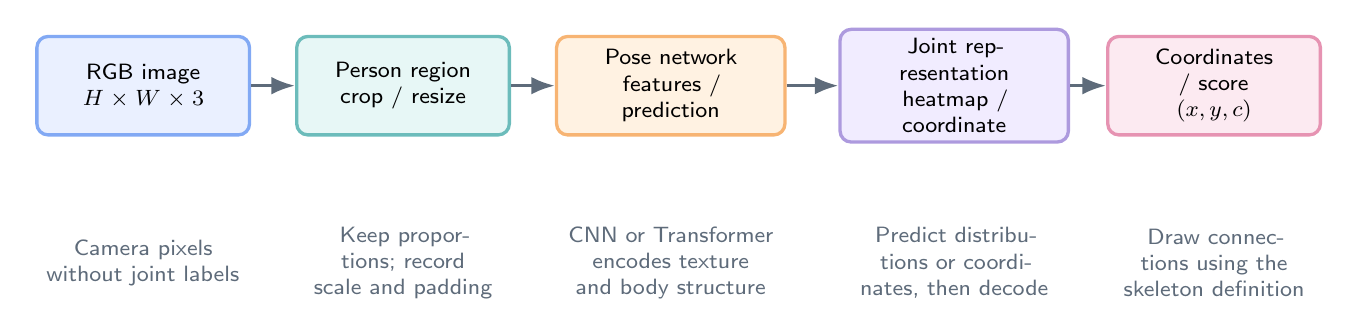
\begin{tikzpicture}[x=1cm,y=1cm,font=\footnotesize]
  \node[draw=Blue!60,fill=BlueSoft,very thick,rounded corners=4pt,minimum width=2.7cm,minimum height=1.25cm,align=center,text width=2.15cm] (img) at (1.5,2.9) {RGB image\\$H\times W\times3$};
  \node[draw=Teal!60,fill=TealSoft,very thick,rounded corners=4pt,minimum width=2.7cm,minimum height=1.25cm,align=center,text width=2.15cm] (person) at (4.8,2.9) {Person region\\crop / resize};
  \node[draw=Orange!65,fill=OrangeSoft,very thick,rounded corners=4pt,minimum width=2.9cm,minimum height=1.25cm,align=center,text width=2.35cm] (net) at (8.2,2.9) {Pose network\\features / prediction};
  \node[draw=Purple!60,fill=PurpleSoft,very thick,rounded corners=4pt,minimum width=2.9cm,minimum height=1.25cm,align=center,text width=2.35cm] (rep) at (11.8,2.9) {Joint representation\\heatmap / coordinate};
  \node[draw=Pink!60,fill=PinkSoft,very thick,rounded corners=4pt,minimum width=2.7cm,minimum height=1.25cm,align=center,text width=2.15cm] (out) at (15.1,2.9) {Coordinates / score\\$(x,y,c)$};
  \draw[arrow] (img)--(person); \draw[arrow] (person)--(net); \draw[arrow] (net)--(rep); \draw[arrow] (rep)--(out);
  \node[align=center,text width=2.7cm,text=Muted] at (1.5,.65) {Camera pixels without joint labels};
  \node[align=center,text width=2.8cm,text=Muted] at (4.8,.65) {Keep proportions; record scale and padding};
  \node[align=center,text width=3.0cm,text=Muted] at (8.2,.65) {CNN or Transformer encodes texture and body structure};
  \node[align=center,text width=3.0cm,text=Muted] at (11.8,.65) {Predict distributions or coordinates, then decode};
  \node[align=center,text width=2.8cm,text=Muted] at (15.1,.65) {Draw connections using the skeleton definition};
\end{tikzpicture}
\end{adjustbox}
\end{center}

\begin{plainBox}
\textbf{Skeleton lines are visualization conventions.}\quad
Models usually output discrete keypoints. Shoulder-to-elbow and elbow-to-wrist lines are drawn using dataset-defined skeleton connections to support interpretation and measurement.
\end{plainBox}

\section{The Pose Inference Pipeline}

\subsection{Step 1: Locate People and Preprocess Images}

A top-down system first detects people, then crops each box to a fixed input aspect ratio. Preprocessing directly affects localization. If a crop excludes a wrist or ankle, the pose model lacks visual evidence. Arbitrary stretching also changes body proportions.

Common preprocessing steps include:
\begin{itemize}
  \item Expand person boxes to keep hands and feet away from crop boundaries.
  \item Use letterboxing or an affine transform to match the model's input ratio.
  \item Convert pixels to tensors and normalize them.
  \item Save the affine matrix to map predicted points back to the original image.
\end{itemize}

\subsection{Step 2: Extract Body Features with the Backbone}

The backbone converts the image into feature maps. Shallow layers retain edges, colors and textures; deeper layers capture relationships between limbs, torso and the whole body. Pose estimation requires both semantic recognition and precise spatial detail, such as the pixels around a wrist.

HRNet maintains high-resolution branches and repeatedly exchanges information with lower-resolution semantic features. ViTPose uses a Vision Transformer encoder and a relatively lightweight decoder. Both address the same requirement: \textbf{joint recognition needs broad context, while accurate localization needs high spatial resolution.}

\subsection{Step 3: Predict a Joint Representation}

Common pose-head outputs include:
\begin{enumerate}
  \item One 2D heatmap per joint.
  \item Directly regressed $(x,y)$ coordinates.
  \item Separate 1D coordinate classifications for $x$ and $y$.
  \item Keypoints together with visibility, depth or joint-connection information.
\end{enumerate}

\clearpage

\section{Heatmaps: Locating Joints from Spatial Distributions}

A heatmap model predicts a 2D distribution for each joint rather than a single point. For $K$ joints, its output can be represented as a $K\times H\times W$ tensor. Channel $k$ describes possible locations of joint $k$ in the input crop. A training target for the right wrist, for example, may use a Gaussian peak around the annotated location:
\[
H_k(x,y)=\exp\left(-\frac{(x-x_k)^2+(y-y_k)^2}{2\sigma^2}\right).
\]
The model predicts $\hat H_k$. MSE, KL divergence or another heatmap loss brings it closer to the target distribution. At inference, coordinates can be decoded using argmax, soft-argmax or an expected value.

\begin{center}
\begin{adjustbox}{max width=\linewidth}
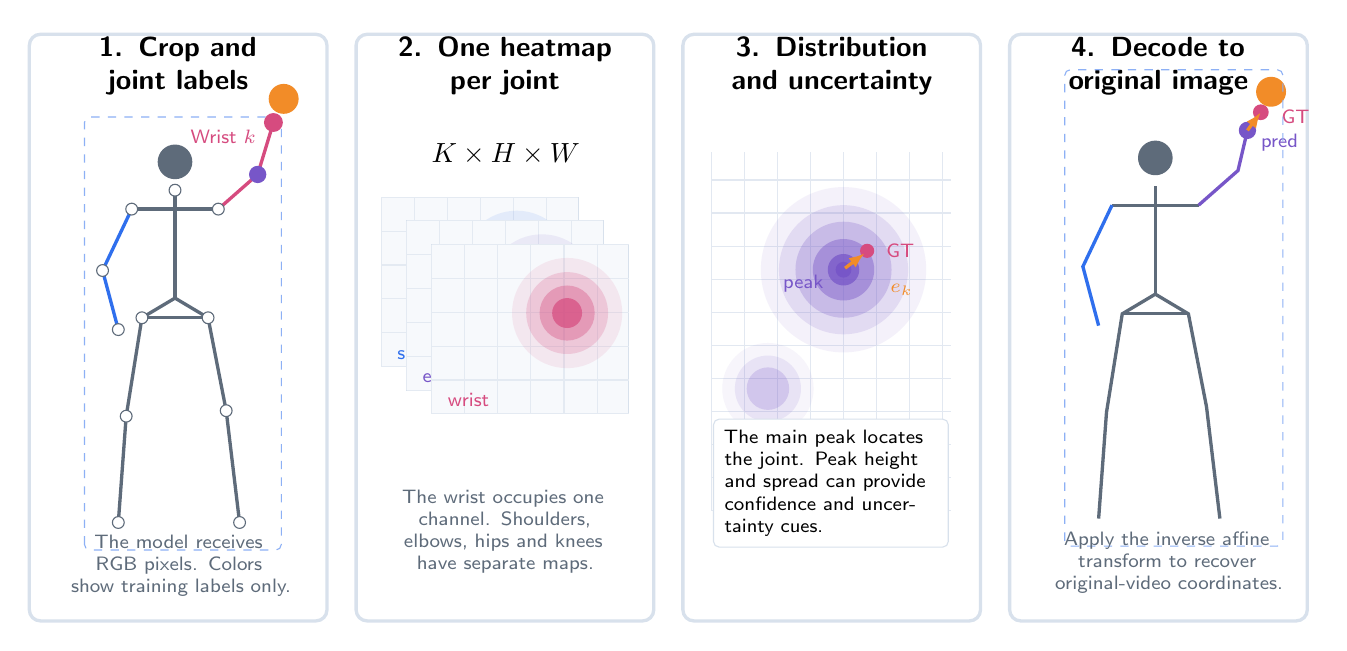
\begin{tikzpicture}[x=1cm,y=1cm,font=\footnotesize]
  \foreach \x/\title in {0/1. Crop and joint labels,4.15/2. One heatmap per joint,8.30/3. Distribution and uncertainty,12.45/4. Decode to original image}{
    \draw[rounded corners=4pt,fill=white,draw=Line,very thick] (\x,0) rectangle ++(3.78,7.45);
    \node[font=\bfseries,align=center,text width=3.45cm] at (\x+1.89,7.05) {\title};
  }

  % Panel 1: full shooting pose
  \begin{scope}[shift={(1.85,1.05)}]
    \draw[Blue!55,dashed,rounded corners=2pt] (-1.15,-.15) rectangle (1.35,5.35);
    \fill[Muted] (0,4.78) circle (.22);
    \coordinate (neck) at (0,4.42); \coordinate (ls) at (-.55,4.18); \coordinate (rs) at (.55,4.18);
    \coordinate (le) at (-.92,3.40); \coordinate (lw) at (-.72,2.65);
    \coordinate (re) at (1.05,4.62); \coordinate (rw) at (1.25,5.28);
    \coordinate (lh) at (-.42,2.80); \coordinate (rh) at (.42,2.80);
    \coordinate (lk) at (-.62,1.55); \coordinate (rk) at (.65,1.62);
    \coordinate (la) at (-.72,.20); \coordinate (ra) at (.82,.20);
    \draw[Muted,very thick] (neck)--(0,3.05); \draw[Muted,very thick] (ls)--(rs);
    \draw[Blue,very thick] (ls)--(le)--(lw); \draw[Pink,very thick] (rs)--(re)--(rw);
    \draw[Muted,very thick] (lh)--(rh); \draw[Muted,very thick] (0,3.05)--(lh)--(lk)--(la); \draw[Muted,very thick] (0,3.05)--(rh)--(rk)--(ra);
    \foreach \p in {neck,ls,le,lw,rs,lh,rh,lk,rk,la,ra}{\fill[white] (\p) circle (.075); \draw[Muted] (\p) circle (.075);}
    \fill[Purple] (re) circle (.11); \fill[Pink] (rw) circle (.12); \fill[Orange] (1.38,5.58) circle (.19);
    \node[font=\scriptsize,anchor=east,text=Pink] at (1.15,5.10) {Wrist $k$};
    \node[font=\scriptsize,text=Muted,align=center,text width=2.8cm] at (.05,-.35) {The model receives RGB pixels. Colors show training labels only.};
  \end{scope}

  % Panel 2: heatmap stack and selected wrist heatmap
  \begin{scope}[shift={(4.47,.78)}]
    \foreach \dx/\dy/\lab/\col in {0/2.45/shoulder/Blue,.32/2.15/elbow/Purple,.64/1.85/wrist/Pink}{
      \draw[fill=Paper,draw=Line] (\dx,\dy) rectangle ++(2.50,2.15);
      \foreach \gx in {0,.42,...,2.5}{\draw[Line!70] (\dx+\gx,\dy)--(\dx+\gx,\dy+2.15);}
      \foreach \gy in {0,.43,...,2.15}{\draw[Line!70] (\dx,\dy+\gy)--(\dx+2.5,\dy+\gy);}
      \foreach \r/\op in {.70/10,.52/20,.35/36,.19/70}{\fill[\col,opacity=\op/100] (\dx+1.72,\dy+1.28) circle (\r);}
      \node[font=\scriptsize,anchor=west,text=\col] at (\dx+.08,\dy+.18) {\lab};
    }
    \node[font=\bfseries] at (1.58,5.15) {$K\times H\times W$};
    \node[font=\scriptsize,text=Muted,align=center,text width=3.0cm] at (1.55,.35) {The wrist occupies one channel. Shoulders, elbows, hips and knees have separate maps.};
  \end{scope}

  % Panel 3: predicted distribution with two modes
  \begin{scope}[shift={(8.66,1.40)}]
    \draw[step=.42,Line!75] (0,0) grid (3.05,4.55);
    \foreach \r/\op in {1.05/8,.82/14,.61/24,.39/42,.20/74}{\fill[Purple,opacity=\op/100] (1.68,3.06) circle (\r);}
    \foreach \r/\op in {.58/6,.42/11,.27/20}{\fill[Purple,opacity=\op/100] (.72,1.55) circle (\r);}
    \fill[Pink] (1.98,3.30) circle (.09); \node[font=\scriptsize,text=Pink,anchor=west] at (2.10,3.30) {GT};
    \fill[Purple] (1.68,3.06) circle (.10); \node[font=\scriptsize,text=Purple,anchor=east] at (1.55,2.88) {peak};
    \draw[Orange,very thick,-{Latex[length=2mm]}] (1.70,3.08)--(1.95,3.27);
    \node[font=\scriptsize,text=Orange] at (2.42,2.80) {$e_k$};
    \node[draw=Line,fill=white,rounded corners=2pt,font=\scriptsize,align=left,text width=2.70cm,inner sep=4pt] at (1.52,.35) {The main peak locates the joint. Peak height and spread can provide confidence and uncertainty cues.};
  \end{scope}

  % Panel 4: decoded overlay and error
  \begin{scope}[shift={(14.30,1.10)}]
    \fill[Muted] (0,4.78) circle (.22);
    \coordinate (n2) at (0,4.42); \coordinate (ls2) at (-.55,4.18); \coordinate (rs2) at (.55,4.18);
    \coordinate (le2) at (-.92,3.40); \coordinate (lw2) at (-.72,2.65);
    \coordinate (re2) at (1.05,4.62); \coordinate (rw2) at (1.17,5.13); \coordinate (rwgt) at (1.34,5.36);
    \coordinate (lh2) at (-.42,2.80); \coordinate (rh2) at (.42,2.80); \coordinate (lk2) at (-.62,1.55); \coordinate (rk2) at (.65,1.62); \coordinate (la2) at (-.72,.20); \coordinate (ra2) at (.82,.20);
    \draw[Muted,very thick] (n2)--(0,3.05); \draw[Muted,very thick] (ls2)--(rs2); \draw[Blue,very thick] (ls2)--(le2)--(lw2); \draw[Purple,very thick] (rs2)--(re2)--(rw2);
    \draw[Muted,very thick] (lh2)--(rh2); \draw[Muted,very thick] (0,3.05)--(lh2)--(lk2)--(la2); \draw[Muted,very thick] (0,3.05)--(rh2)--(rk2)--(ra2);
    \fill[Purple] (rw2) circle (.11); \fill[Pink] (rwgt) circle (.10); \draw[Orange,very thick,-{Latex[length=2mm]}] (rw2)--(rwgt);
    \fill[Orange] (1.47,5.62) circle (.19);
    \node[font=\scriptsize,anchor=west,text=Purple] at (1.22,4.98) {pred}; \node[font=\scriptsize,anchor=west,text=Pink] at (1.48,5.30) {GT};
    \draw[Blue!55,dashed,rounded corners=2pt] (-1.15,-.15) rectangle (1.62,5.90);
    \node[font=\scriptsize,text=Muted,align=center,text width=3.0cm] at (.15,-.36) {Apply the inverse affine transform to recover original-video coordinates.};
  \end{scope}
\end{tikzpicture}
\end{adjustbox}
\end{center}

\begin{plainBox}
\textbf{Reading the diagram:}\quad
Each joint has its own heatmap channel. Peaks, spread and secondary modes convey location and uncertainty. Decoded coordinates must be transformed back to the original image before combining them with player tracks, ball positions and the full skeleton.
\end{plainBox}

\subsection{Heatmap Resolution and Quantization Error}


For a $256\times192$ input and a $64\times48$ output heatmap, each heatmap pixel corresponds to roughly $4\times4$ input pixels. Plain argmax restricts coordinates to a discrete grid. Quarter-pixel correction, soft-argmax, DARK decoding and integral regression can reduce this quantization error.

Higher heatmap resolution can improve localization but increases memory use and computation. A distant player's wrist may occupy only a few original pixels. Cropping and downscaling can discard information that no decoder can recover.

\section{Coordinate Regression and Classification}

\begin{tabularx}{\textwidth}{>{\bfseries\RaggedRight}p{3.5cm} Y Y}
\toprule
Representation & Method & Properties \\
\midrule
2D heatmap & Predict an $H\times W$ map for each joint & Intuitive and effective; high-resolution maps cost more, and discrete grids introduce quantization error.\\
Direct regression & Output $2K$ coordinates directly & Compact output, but precise localization from global features can be difficult.\\
Integral regression & Take a differentiable expectation over a heatmap & Combines heatmaps with continuous coordinates and avoids a hard, non-differentiable argmax.\\
Coordinate classification & Predict separate binned 1D distributions for $x$ and $y$ & Avoids a full 2D heatmap. SimCC and RTMPose use this approach to balance accuracy and efficiency.\\
\bottomrule
\end{tabularx}

\begin{plainBox}
\textbf{When choosing a representation, consider:}\quad
Input resolution, person size in the image, deployment speed, localization accuracy and whether later measurements, such as wrist velocity or angle differences, are sensitive to jitter.
\end{plainBox}

\clearpage
\section{Multi-Person Pose: Top-Down and Bottom-Up Methods}

A multi-person system must locate joints and assign them to the correct people. Two common approaches address this task.

\begin{center}
\begin{adjustbox}{max width=\linewidth}
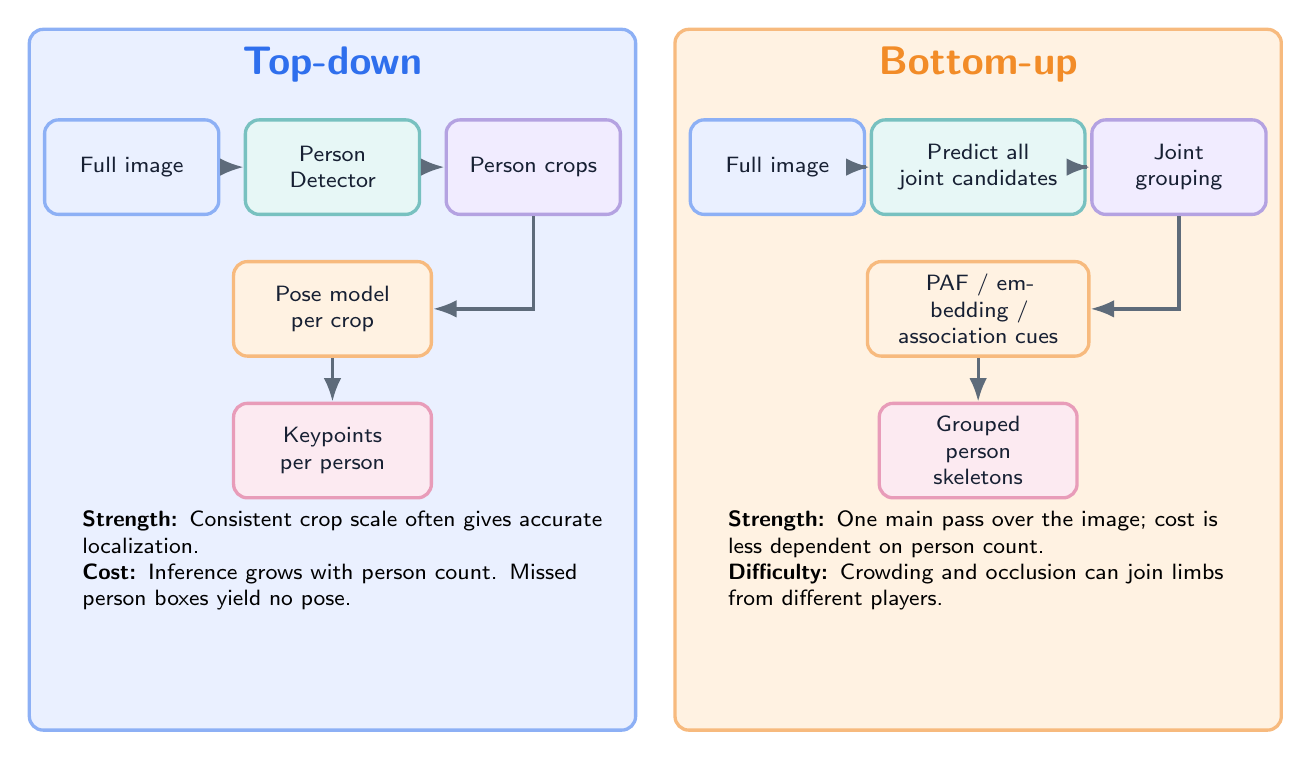
\begin{tikzpicture}[x=1cm,y=1cm,font=\footnotesize]
  \draw[rounded corners=5pt,fill=BlueSoft,draw=Blue!55,very thick] (0,-1.8) rectangle (7.7,7.1);
  \draw[rounded corners=5pt,fill=OrangeSoft,draw=Orange!60,very thick] (8.2,-1.8) rectangle (15.9,7.1);
  \node[font=\bfseries\Large,text=Blue] at (3.85,6.65) {Top-down};
  \node[font=\bfseries\Large,text=Orange] at (12.05,6.65) {Bottom-up};

  \node[flowblue,minimum width=2.2cm,text width=1.65cm] (tdimg) at (1.3,5.35) {Full image};
  \node[flowteal,minimum width=2.2cm,text width=1.65cm] (det) at (3.85,5.35) {Person\\Detector};
  \node[flowpurple,minimum width=2.2cm,text width=1.65cm] (crop) at (6.4,5.35) {Person crops};
  \draw[arrow] (tdimg)--(det); \draw[arrow] (det)--(crop);
  \node[floworange,minimum width=2.5cm,text width=1.95cm] (pose1) at (3.85,3.55) {Pose model\\per crop};
  \draw[arrow] (crop.south) |- (pose1.east);
  \node[flowpink,minimum width=2.5cm,text width=1.95cm] (tdout) at (3.85,1.75) {Keypoints\\per person};
  \draw[arrow] (pose1)--(tdout);
  \node[align=left,text width=6.6cm,anchor=north west] at (.55,1.1) {\textbf{Strength:} Consistent crop scale often gives accurate localization.\\\textbf{Cost:} Inference grows with person count. Missed person boxes yield no pose.};

  \node[flowblue,minimum width=2.2cm,text width=1.65cm] (buimg) at (9.5,5.35) {Full image};
  \node[flowteal,minimum width=2.7cm,text width=2.15cm] (allkp) at (12.05,5.35) {Predict all\\joint candidates};
  \node[flowpurple,minimum width=2.2cm,text width=1.65cm] (assoc) at (14.6,5.35) {Joint\\grouping};
  \draw[arrow] (buimg)--(allkp); \draw[arrow] (allkp)--(assoc);
  \node[floworange,minimum width=2.8cm,text width=2.25cm] (paf) at (12.05,3.55) {PAF / embedding /\\association cues};
  \draw[arrow] (assoc.south) |- (paf.east);
  \node[flowpink,minimum width=2.5cm,text width=1.95cm] (buout) at (12.05,1.75) {Grouped\\person skeletons};
  \draw[arrow] (paf)--(buout);
  \node[align=left,text width=6.6cm,anchor=north west] at (8.75,1.1) {\textbf{Strength:} One main pass over the image; cost is less dependent on person count.\\\textbf{Difficulty:} Crowding and occlusion can join limbs from different players.};
\end{tikzpicture}
\end{adjustbox}
\end{center}

Basketball has a relatively fixed player count but frequent occlusion. Top-down methods integrate readily with detectors and trackers: crop a tracked player, then estimate that player's pose. In distant full-court footage, however, the crop may contain too few effective pixels to locate wrists and ankles, even when the player is detected.

\section{Representative Pose Models}

\begin{tabularx}{\textwidth}{>{\bfseries\RaggedRight}p{2.7cm} p{3.1cm} Y Y}
\toprule
Model & Approach & Main design & Basketball considerations \\
\midrule
OpenPose & Bottom-up & Joint heatmaps and part affinity fields, followed by grouping. & Handles multiple people; small or overlapping players make grouping harder.\\
HRNet & Often a top-down backbone & Maintains high-resolution branches with repeated multi-scale fusion. & Supports precise localization; cost depends on model and input size.\\
BlazePose & Single-person detection and tracking & Lightweight, real-time mobile design with 33 landmarks. & Suitable for close-up training views; full-court multi-person capability should not be assumed.\\
ViTPose & Top-down / Transformer & Plain Vision Transformer encoder and a lightweight keypoint decoder. & Flexible model scale and accuracy; assess cost for the chosen backbone.\\
RTMPose & Real-time top-down & Integrates training, architecture and deployment, often with coordinate classification. & Useful for high-throughput multi-person pipelines; crop resolution remains a limit.\\
\bottomrule
\end{tabularx}



\section{Visibility, Occlusion and Joint Confidence}

A pose model supplies joint coordinates with varying reliability, not an invariably complete skeleton. Ball occlusion, overlapping limbs, image boundaries and tight crops can make wrists, elbows, knees or ankles unreliable even when the person box is correct. Angle and event analysis must therefore use confidence and visibility rules alongside coordinates.

\begin{center}
\begin{adjustbox}{max width=\linewidth}
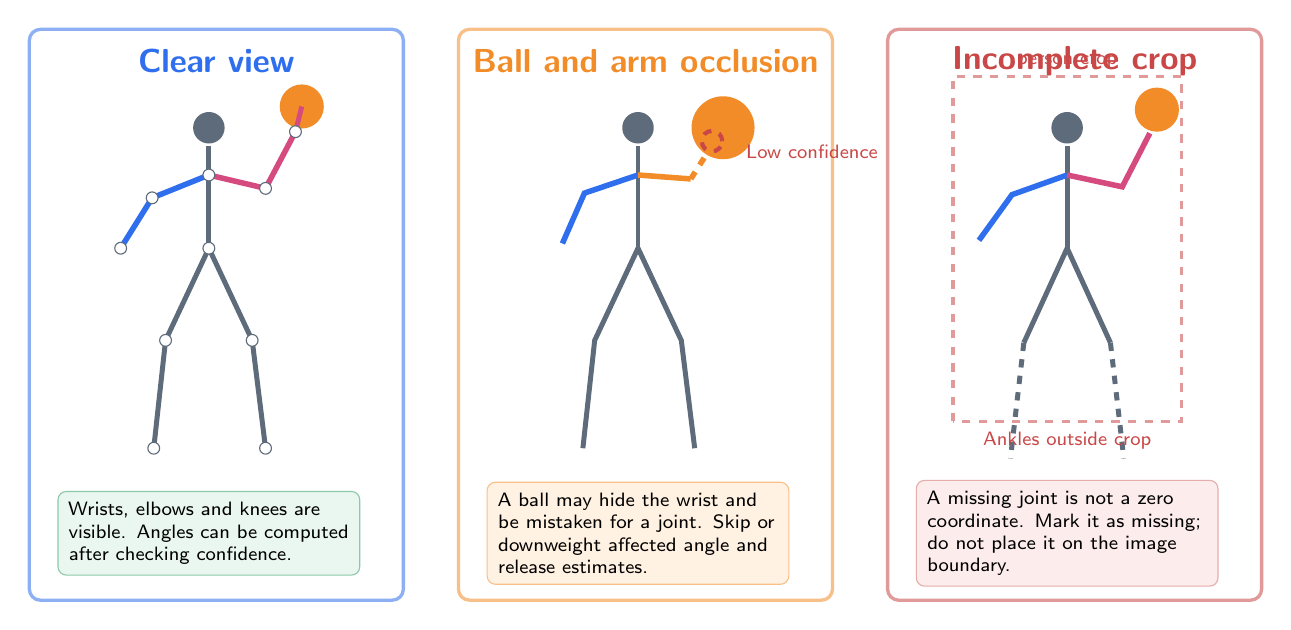
\begin{tikzpicture}[x=1cm,y=1cm,font=\footnotesize]
  \foreach \x/\ttl/\col in {0/Clear view/Blue,5.45/Ball and arm occlusion/Orange,10.90/Incomplete crop/Red}{
    \draw[rounded corners=4pt,fill=white,draw=\col!55,line width=1.2pt] (\x,-.7) rectangle ++(4.75,7.25);
    \node[font=\bfseries\large,text=\col] at (\x+2.375,6.15) {\ttl};
  }

  \begin{scope}[shift={(2.28,1.05)}]
    \fill[Muted] (0,4.25) circle (.20);
    \draw[Muted,line width=1.8pt] (0,4.02)--(0,2.72);
    \draw[Blue,line width=2pt] (0,3.65)--(-.72,3.36)--(-1.12,2.72);
    \draw[Pink,line width=2pt] (0,3.65)--(.72,3.48)--(1.10,4.20);
    \draw[Muted,line width=1.8pt] (0,2.72)--(-.55,1.55)--(-.70,.18);
    \draw[Muted,line width=1.8pt] (0,2.72)--(.55,1.55)--(.72,.18);
    \fill[Orange] (1.18,4.52) circle (.28);
    \draw[Pink,line width=1.8pt] (1.10,4.20)--(1.18,4.52);
    \foreach \p in {(0,3.65),(-.72,3.36),(-1.12,2.72),(.72,3.48),(1.10,4.20),(0,2.72),(-.55,1.55),(.55,1.55),(-.70,.18),(.72,.18)}
      {\fill[white] \p circle (.075); \draw[Muted] \p circle (.075);}
    \node[draw=Green!55,fill=GreenSoft,rounded corners=3pt,font=\scriptsize,align=left,text width=3.55cm,inner sep=4pt] at (0,-.9)
      {Wrists, elbows and knees are visible. Angles can be computed after checking confidence.};
  \end{scope}

  \begin{scope}[shift={(7.73,1.05)}]
    \fill[Muted] (0,4.25) circle (.20);
    \draw[Muted,line width=1.8pt] (0,4.02)--(0,2.72);
    \draw[Blue,line width=2pt] (0,3.65)--(-.68,3.42)--(-.96,2.78);
    \draw[Orange,line width=2pt] (0,3.65)--(.67,3.60);
    \draw[Orange,dashed,line width=2pt] (.67,3.60)--(1.04,4.18);
    \draw[Muted,line width=1.8pt] (0,2.72)--(-.55,1.55)--(-.70,.18);
    \draw[Muted,line width=1.8pt] (0,2.72)--(.55,1.55)--(.72,.18);
    \fill[Orange] (1.08,4.25) circle (.40);
    \draw[Red,dashed,line width=1.5pt] (.94,4.08) circle (.13);
    \node[font=\scriptsize,text=Red,anchor=west] at (1.25,3.95) {Low confidence};
    \node[draw=Orange!55,fill=OrangeSoft,rounded corners=3pt,font=\scriptsize,align=left,text width=3.55cm,inner sep=4pt] at (0,-.9)
      {A ball may hide the wrist and be mistaken for a joint. Skip or downweight affected angle and release estimates.};
  \end{scope}

  \begin{scope}[shift={(13.18,1.05)}]
    \draw[Red!55,dashed,line width=1.2pt] (-1.45,.52) rectangle (1.45,4.90);
    \node[font=\scriptsize,text=Red] at (0,5.08) {person crop};
    \fill[Muted] (0,4.25) circle (.20);
    \draw[Muted,line width=1.8pt] (0,4.02)--(0,2.72);
    \draw[Blue,line width=2pt] (0,3.65)--(-.70,3.40)--(-1.12,2.82);
    \draw[Pink,line width=2pt] (0,3.65)--(.70,3.50)--(1.05,4.18);
    \fill[Orange] (1.14,4.48) circle (.28);
    \draw[Muted,line width=1.8pt] (0,2.72)--(-.55,1.52);
    \draw[Muted,dashed,line width=1.8pt] (-.55,1.52)--(-.72,.05);
    \draw[Muted,line width=1.8pt] (0,2.72)--(.55,1.52);
    \draw[Muted,dashed,line width=1.8pt] (.55,1.52)--(.72,.05);
    \node[font=\scriptsize,text=Red] at (0,.28) {Ankles outside crop};
    \node[draw=Red!45,fill=RedSoft,rounded corners=3pt,font=\scriptsize,align=left,text width=3.55cm,inner sep=4pt] at (0,-.9)
      {A missing joint is not a zero coordinate. Mark it as missing; do not place it on the image boundary.};
  \end{scope}
\end{tikzpicture}
\end{adjustbox}
\end{center}

\subsection{Using Confidence in Measurements}

A joint commonly has output $(x_k,y_k,s_k)$, where $s_k$ is confidence. Check every joint used by an angle or event rule:

\begin{enumerate}
  \item If any shoulder, elbow or wrist score is below threshold, mark the elbow angle as missing for that frame.
  \item A one- or two-frame gap may be interpolated using nearby frames and velocity limits. Retain missing values during long occlusions.
  \item Reduce trust near crop boundaries, where truncation can cause systematic bias.
  \item Use confidence in temporal smoothing so reliable observations carry more weight.
\end{enumerate}

\begin{plainBox}
\textbf{Suggested data representation:}\quad
Store at least \texttt{x}, \texttt{y}, \texttt{confidence}, \texttt{visible/missing} and the original image size for each joint. Use an explicit missing-value mask rather than $(0,0)$, which can create false motion in averages and angle calculations.
\end{plainBox}

\section{Pose in Video: Tracking and Temporal Consistency}

Single-image pose models usually process frames independently. Blur, occlusion and changing detector crops can cause joint jitter. Video systems often add:
\begin{itemize}
  \item Player track IDs to associate crops with the same person.
  \item Previous-frame keypoints to narrow the search region.
  \item EMA, Savitzky--Golay or Kalman filtering to reduce high-frequency jitter.
  \item Temporal convolutions, RNNs or video Transformers to learn temporal relationships.
  \item Missing values for unreliable joints, without arbitrary connections or imputation.
\end{itemize}

\begin{center}
\begin{adjustbox}{max width=\linewidth}
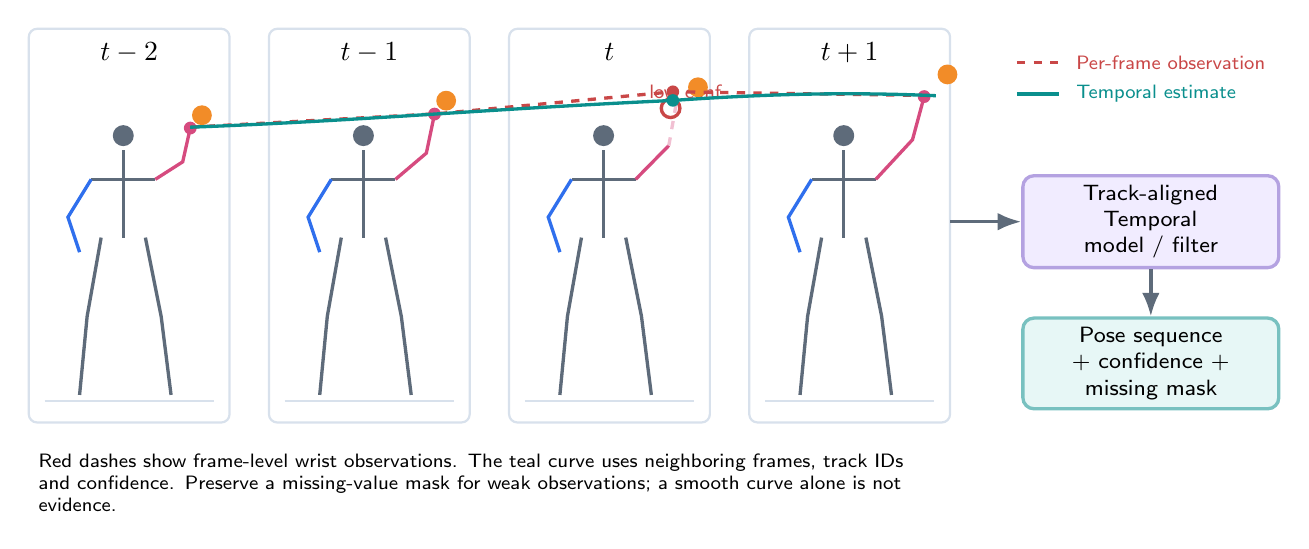
\begin{tikzpicture}[x=1cm,y=1cm,font=\footnotesize]
  \foreach \x/\lab in {0/$t-2$,3.05/$t-1$,6.10/$t$,9.15/$t+1$}{
    \draw[rounded corners=3pt,fill=white,draw=Line,thick] (\x,1.35) rectangle ++(2.55,5.00);
    \node[font=\bfseries] at (\x+1.275,6.05) {\lab};
    \draw[Line,thick] (\x+.20,1.62)--(\x+2.35,1.62);
  }
  % frame t-2
  \begin{scope}[shift={(1.20,1.70)},scale=.74]
    \fill[Muted] (0,4.45) circle (.18); \draw[Muted,very thick] (0,4.20)--(0,2.70); \draw[Muted,very thick] (-.55,3.70)--(.55,3.70);
    \draw[Blue,very thick] (-.55,3.70)--(-.95,3.05)--(-.75,2.45); \draw[Pink,very thick] (.55,3.70)--(1.02,4.00)--(1.15,4.58);
    \draw[Muted,very thick] (-.38,2.70)--(-.62,1.35)--(-.75,0); \draw[Muted,very thick] (.38,2.70)--(.65,1.35)--(.82,0);
    \fill[Pink] (1.15,4.58) circle (.11); \fill[Orange] (1.35,4.80) circle (.17);
  \end{scope}
  % t-1
  \begin{scope}[shift={(4.25,1.70)},scale=.74]
    \fill[Muted] (0,4.45) circle (.18); \draw[Muted,very thick] (0,4.20)--(0,2.70); \draw[Muted,very thick] (-.55,3.70)--(.55,3.70);
    \draw[Blue,very thick] (-.55,3.70)--(-.95,3.05)--(-.75,2.45); \draw[Pink,very thick] (.55,3.70)--(1.08,4.15)--(1.22,4.82);
    \draw[Muted,very thick] (-.38,2.70)--(-.62,1.35)--(-.75,0); \draw[Muted,very thick] (.38,2.70)--(.65,1.35)--(.82,0);
    \fill[Pink] (1.22,4.82) circle (.11); \fill[Orange] (1.42,5.05) circle (.17);
  \end{scope}
  % t occluded / low confidence wrist
  \begin{scope}[shift={(7.30,1.70)},scale=.74]
    \fill[Muted] (0,4.45) circle (.18); \draw[Muted,very thick] (0,4.20)--(0,2.70); \draw[Muted,very thick] (-.55,3.70)--(.55,3.70);
    \draw[Blue,very thick] (-.55,3.70)--(-.95,3.05)--(-.75,2.45); \draw[Pink,very thick] (.55,3.70)--(1.12,4.28); \draw[Pink!35,dashed,very thick] (1.12,4.28)--(1.25,5.02);
    \draw[Muted,very thick] (-.38,2.70)--(-.62,1.35)--(-.75,0); \draw[Muted,very thick] (.38,2.70)--(.65,1.35)--(.82,0);
    \draw[Red,very thick] (1.15,4.92) circle (.16); \node[text=Red,font=\scriptsize] at (1.45,5.20) {low conf.};
    \fill[Orange] (1.62,5.28) circle (.17);
  \end{scope}
  % t+1
  \begin{scope}[shift={(10.35,1.70)},scale=.74]
    \fill[Muted] (0,4.45) circle (.18); \draw[Muted,very thick] (0,4.20)--(0,2.70); \draw[Muted,very thick] (-.55,3.70)--(.55,3.70);
    \draw[Blue,very thick] (-.55,3.70)--(-.95,3.05)--(-.75,2.45); \draw[Pink,very thick] (.55,3.70)--(1.18,4.38)--(1.38,5.12);
    \draw[Muted,very thick] (-.38,2.70)--(-.62,1.35)--(-.75,0); \draw[Muted,very thick] (.38,2.70)--(.65,1.35)--(.82,0);
    \fill[Pink] (1.38,5.12) circle (.11); \fill[Orange] (1.78,5.50) circle (.17);
  \end{scope}

  % raw and filtered wrist trajectory across frames
  \draw[Red,dashed,very thick] (2.05,5.10)--(5.18,5.27)--(8.18,5.55)--(11.52,5.50);
  \draw[Teal,very thick] (2.05,5.10)..controls(4.20,5.18) and (5.80,5.33)..(8.18,5.44)..controls(9.35,5.52) and (10.35,5.55)..(11.52,5.50);
  \fill[Red] (8.18,5.55) circle (.08); \fill[Teal] (8.18,5.44) circle (.08);
  \draw[Red,dashed,very thick] (12.55,5.92)--(13.08,5.92);
  \node[font=\scriptsize,text=Red,anchor=west] at (13.18,5.92) {Per-frame observation};
  \draw[Teal,very thick] (12.55,5.52)--(13.08,5.52);
  \node[font=\scriptsize,text=Teal,anchor=west] at (13.18,5.52) {Temporal estimate};

  % temporal fusion box and outputs
  \node[draw=Purple!55,fill=PurpleSoft,rounded corners=4pt,very thick,minimum width=3.25cm,minimum height=1.05cm,align=center,text width=2.70cm] (temp) at (14.25,3.90) {Track-aligned\\Temporal model / filter};
  \draw[arrow] (11.70,3.90)--(temp);
  \node[draw=Teal!55,fill=TealSoft,rounded corners=4pt,very thick,minimum width=3.25cm,minimum height=1.05cm,align=center,text width=2.70cm] (stable) at (14.25,2.10) {Pose sequence\\+ confidence + missing mask};
  \draw[arrow] (temp)--(stable);
  \node[align=left,text width=11.2cm,anchor=west,font=\scriptsize] at (0,.58) {Red dashes show frame-level wrist observations. The teal curve uses neighboring frames, track IDs and confidence. Preserve a missing-value mask for weak observations; a smooth curve alone is not evidence.};
\end{tikzpicture}
\end{adjustbox}
\end{center}

\begin{plainBox}
\textbf{Temporal models must preserve meaningful motion.}\quad
A shot release includes rapid acceleration and direction changes. Excessive smoothing can delay the estimated release frame and reduce peak velocity. Evaluate jitter, event-timing error and preservation of motion peaks together.
\end{plainBox}

\section{Measuring Shooting Motion from Keypoints}


\subsection{Joint Angles from Three Points}

For shoulder $A$, elbow $B$ and wrist $C$, the angle at $B$ is:
\[
\theta=\cos^{-1}\left(
\frac{(A-B)\cdot(C-B)}{\|A-B\|_2\|C-B\|_2}
\right).
\]

\begin{center}
\begin{adjustbox}{max width=\linewidth}
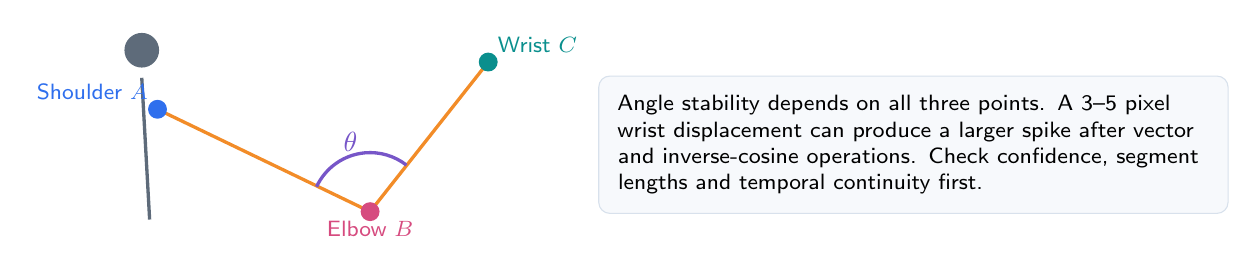
\begin{tikzpicture}[x=1cm,y=1cm,font=\footnotesize]
  \coordinate (s) at (2.0,3.7); \coordinate (e) at (4.7,2.4); \coordinate (w) at (6.2,4.3);
  \draw[Muted,very thick] (1.8,4.1)--(1.9,2.3); \fill[Muted] (1.8,4.45) circle (.22);
  \draw[Orange,very thick] (s)--(e)--(w);
  \fill[Blue] (s) circle (.12) node[above left] {Shoulder $A$};
  \fill[Pink] (e) circle (.12) node[below] {Elbow $B$};
  \fill[Teal] (w) circle (.12) node[above right] {Wrist $C$};
  \draw[Purple,very thick] ($(e)+(155:0.75)$) arc[start angle=155,end angle=52,radius=.75];
  \node[Purple,font=\bfseries] at (4.45,3.28) {$\theta$};
  \node[draw=Line,fill=Paper,rounded corners=4pt,text width=7.5cm,align=left,inner sep=7pt] at (11.6,3.25) {Angle stability depends on all three points. A 3--5 pixel wrist displacement can produce a larger spike after vector and inverse-cosine operations. Check confidence, segment lengths and temporal continuity first.};
\end{tikzpicture}
\end{adjustbox}
\end{center}

\subsection{Ball-to-Wrist Relationships and Release Detection}

Release is an event, not a standard keypoint output by a pose model. Estimating it generally combines pose, ball detection or tracking, and temporal rules:
\begin{enumerate}
  \item Identify the ball handler's track and locate the shooting wrist.
  \item Track the ball center and compute its distance from the wrist.
  \item Check for sustained separation across frames rather than a single-frame jump.
  \item Also inspect ball velocity direction, elbow extension and wrist follow-through.
  \item Compare candidate intervals with manual labels and report timing error and confidence.
\end{enumerate}

\begin{center}
\begin{adjustbox}{max width=\linewidth}
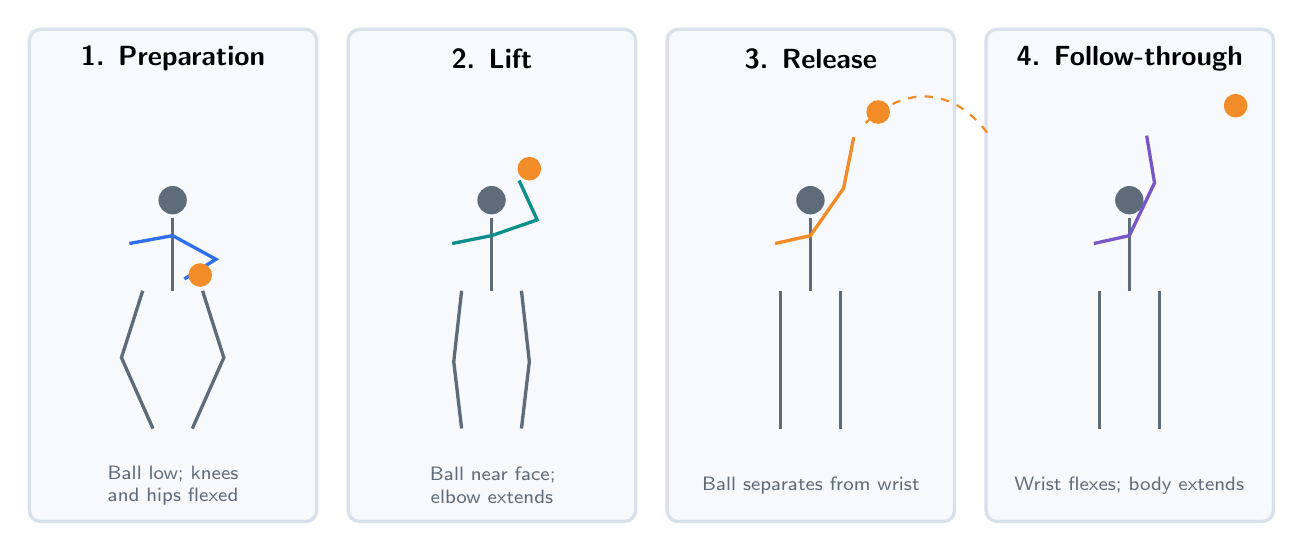
\begin{tikzpicture}[x=1cm,y=1cm,font=\footnotesize]
\foreach \x/\title/\subtitle in {0/1. Preparation/Ball low; knees and hips flexed,4.05/2. Lift/Ball near face; elbow extends,8.10/3. Release/Ball separates from wrist,12.15/4. Follow-through/Wrist flexes; body extends}{
  \draw[rounded corners=4pt,fill=Paper,draw=Line,very thick] (\x,0) rectangle ++(3.65,6.25);
  \node[font=\bfseries] at (\x+1.825,5.88) {\title};
  \node[align=center,text width=3.1cm,text=Muted,font=\scriptsize] at (\x+1.825,.46) {\subtitle};
}
\begin{scope}[shift={(1.82,1.18)}]
  \fill[Muted] (0,2.9) circle (.18); \draw[Muted,very thick] (0,2.68)--(0,1.75);
  \draw[Blue,very thick] (-.55,2.35)--(0,2.45)--(.55,2.15)--(.15,1.9); \draw[Muted,very thick] (-.38,1.75)--(-.65,.9)--(-.25,0); \draw[Muted,very thick] (.38,1.75)--(.65,.9)--(.25,0); \fill[Orange] (.35,1.95) circle (.15);
\end{scope}
\begin{scope}[shift={(5.87,1.18)}]
  \fill[Muted] (0,2.9) circle (.18); \draw[Muted,very thick] (0,2.68)--(0,1.75);
  \draw[Teal,very thick] (-.50,2.35)--(0,2.45)--(.58,2.65)--(.35,3.15); \draw[Muted,very thick] (-.38,1.75)--(-.48,.85)--(-.38,0); \draw[Muted,very thick] (.38,1.75)--(.48,.85)--(.38,0); \fill[Orange] (.48,3.3) circle (.15);
\end{scope}
\begin{scope}[shift={(9.92,1.18)}]
  \fill[Muted] (0,2.9) circle (.18); \draw[Muted,very thick] (0,2.68)--(0,1.75);
  \draw[Orange,very thick] (-.45,2.35)--(0,2.45)--(.42,3.05)--(.55,3.7); \draw[Muted,very thick] (-.38,1.75)--(-.38,.85)--(-.38,0); \draw[Muted,very thick] (.38,1.75)--(.38,.85)--(.38,0); \fill[Orange] (.86,4.02) circle (.15);
  \draw[Orange,dashed,thick] (.70,3.88) .. controls (1.2,4.35) and (1.8,4.35) .. (2.25,3.75);
\end{scope}
\begin{scope}[shift={(13.97,1.18)}]
  \fill[Muted] (0,2.9) circle (.18); \draw[Muted,very thick] (0,2.68)--(0,1.75);
  \draw[Purple,very thick] (-.45,2.35)--(0,2.45)--(.32,3.12)--(.22,3.72); \draw[Muted,very thick] (-.38,1.75)--(-.38,.85)--(-.38,0); \draw[Muted,very thick] (.38,1.75)--(.38,.85)--(.38,0); \fill[Orange] (1.35,4.10) circle (.15);
\end{scope}
\end{tikzpicture}
\end{adjustbox}
\end{center}

\begin{pseudoBox}
FOR each tracked player and each frame
  transform the player crop and run the pose model
  map keypoints back to the original image
  reject or mask low-confidence joints
  associate the ball track with the shooting hand
  compute joint angles, ball-to-wrist distance and temporal derivatives
FIND a stable release interval using several consecutive frames
RETURN the interval, supporting signals and confidence
\end{pseudoBox}

\section{Pose Evaluation Metrics}

\begin{tabularx}{\textwidth}{>{\bfseries\RaggedRight}p{3.0cm} Y Y}
\toprule
Metric & Measurement & What to check \\
\midrule
PCK & Fraction of predicted joints within a normalized distance threshold of ground truth & Is distance normalized by box, head or torso size? What threshold is used?\\
OKS & Keypoint similarity adjusted for person scale and joint-specific tolerance & COCO keypoint AP uses OKS; $\kappa$ differs across joints.\\
Keypoint AP / AR & Precision and recall across several OKS thresholds & Depends on person detection, joint localization and assignment to people.\\
MPJPE & Mean Euclidean error of 3D joints & Root, scale and Procrustes alignment produce different values; do not mix protocols.\\
Temporal error & Error in release, event boundaries or peak timing & Report frames or milliseconds, video FPS and annotation agreement.\\
\bottomrule
\end{tabularx}

\begin{takeawayBox}
The main pipeline is \textbf{person regions and coordinate transforms $\rightarrow$ feature extraction $\rightarrow$ joint representation $\rightarrow$ coordinate decoding $\rightarrow$ temporal and geometric measurements}. Architecture is only one factor. Person scale, viewing angle, crop quality, heatmap resolution, joint grouping and temporal consistency jointly determine reliability.
\end{takeawayBox}


% ================================================================
% DAY 5
% ================================================================
\chapter{Project Proposals: From Problem Definition to Validation}

\begin{heroBox}
\textbf{Main question:}\quad
How can the detection, tracking, geometry, pose and event modules from Days 1--4 become a proposal with a clear problem, traceable data, comparable methods and verifiable results?
\end{heroBox}

\section{Start with the Use Case and Research Question}

\begin{conceptBox}
``Build a basketball analysis system with YOLO, ByteTrack and MediaPipe'' lists technologies but does not yet define a project. A proposal must identify the intended users or research subjects, data context, system outputs and validation method.
\end{conceptBox}

An evaluable research question usually specifies:

\begin{itemize}
  \item \textbf{Users:} Players, coaches, analysts, broadcast teams or researchers.
  \item \textbf{Setting:} Fixed camera, broadcast footage, individual training or fixed half-court video.
  \item \textbf{Inputs:} RGB video, court keypoints, rosters and required calibration data.
  \item \textbf{Outputs:} Positions, identities, teams, events, movement measurements or reports.
  \item \textbf{Comparison:} Which baseline should be improved, and on which metrics?
  \item \textbf{Limits:} Which viewing angles, lighting or occlusion conditions are unsupported?
\end{itemize}

\begin{plainBox}
\textbf{Too broad:} Use AI to analyze players.\\
\textbf{Testable question:} With a fixed half-court camera, does track-level voting on jersey features reduce team-label switching compared with frame-level K-means?\\
\textbf{Experiment:} Across three test games with different jerseys and lighting, compare team accuracy and switching rates for frame-level HSV, frame-level deep embeddings and track-level temporal voting.
\end{plainBox}

\clearpage
\section{Architecture Diagrams Should Show Data Transformations}

Show how each module changes the data, rather than listing model names alone. Module names, input/output fields and coordinate units should agree. This lets teachers and students trace an implausible result back through the pipeline.

\begin{center}
\begin{adjustbox}{max width=\linewidth}
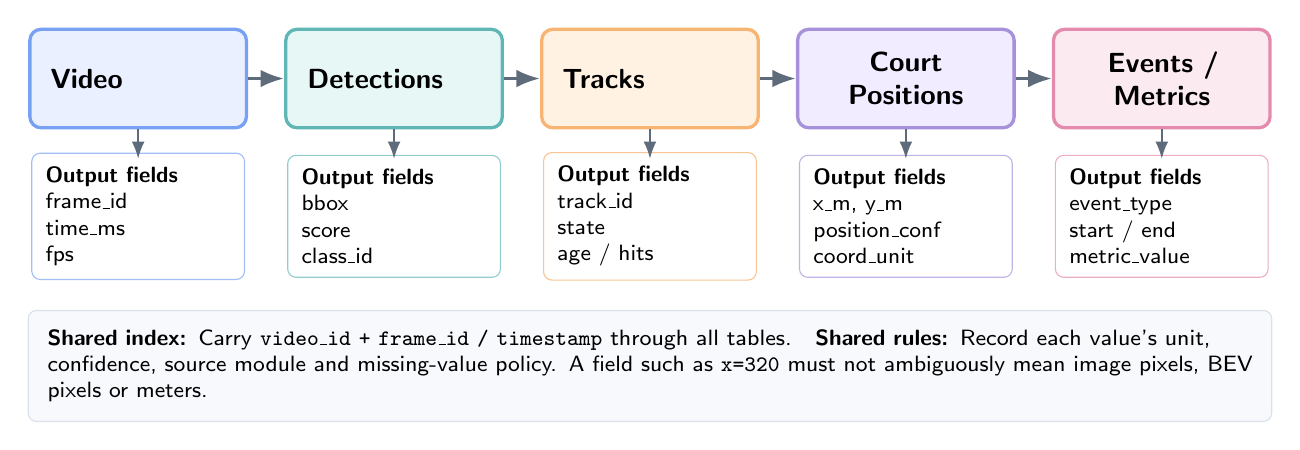
\begin{tikzpicture}[x=1cm,y=1cm,font=\footnotesize]
  \node[draw=Blue!65,fill=BlueSoft,very thick,rounded corners=4pt,minimum width=2.75cm,minimum height=1.25cm,font=\bfseries,text width=2.20cm] (video) at (1.375,3.2) {Video};
  \node[draw=Teal!65,fill=TealSoft,very thick,rounded corners=4pt,minimum width=2.75cm,minimum height=1.25cm,font=\bfseries,text width=2.20cm] (det) at (4.625,3.2) {Detections};
  \node[draw=Orange!65,fill=OrangeSoft,very thick,rounded corners=4pt,minimum width=2.75cm,minimum height=1.25cm,font=\bfseries,text width=2.20cm] (trk) at (7.875,3.2) {Tracks};
  \node[draw=Purple!65,fill=PurpleSoft,very thick,rounded corners=4pt,minimum width=2.75cm,minimum height=1.25cm,align=center,font=\bfseries,text width=2.20cm] (court) at (11.125,3.2) {Court\\Positions};
  \node[draw=Pink!65,fill=PinkSoft,very thick,rounded corners=4pt,minimum width=2.75cm,minimum height=1.25cm,align=center,font=\bfseries,text width=2.20cm] (event) at (14.375,3.2) {Events /\\Metrics};
  \draw[arrow] (video)--(det); \draw[arrow] (det)--(trk); \draw[arrow] (trk)--(court); \draw[arrow] (court)--(event);
  \node[draw=Blue!45,fill=white,rounded corners=3pt,text width=2.35cm,align=left,inner sep=5pt] at (1.375,1.45) {\textbf{Output fields}\\frame\_id\\time\_ms\\fps};
  \node[draw=Teal!45,fill=white,rounded corners=3pt,text width=2.35cm,align=left,inner sep=5pt] at (4.625,1.45) {\textbf{Output fields}\\bbox\\score\\class\_id};
  \node[draw=Orange!50,fill=white,rounded corners=3pt,text width=2.35cm,align=left,inner sep=5pt] at (7.875,1.45) {\textbf{Output fields}\\track\_id\\state\\age / hits};
  \node[draw=Purple!45,fill=white,rounded corners=3pt,text width=2.35cm,align=left,inner sep=5pt] at (11.125,1.45) {\textbf{Output fields}\\x\_m, y\_m\\position\_conf\\coord\_unit};
  \node[draw=Pink!45,fill=white,rounded corners=3pt,text width=2.35cm,align=left,inner sep=5pt] at (14.375,1.45) {\textbf{Output fields}\\event\_type\\start / end\\metric\_value};
  \draw[thinArrow] (video.south)--(1.375,2.18); \draw[thinArrow] (det.south)--(4.625,2.18); \draw[thinArrow] (trk.south)--(7.875,2.18); \draw[thinArrow] (court.south)--(11.125,2.18); \draw[thinArrow] (event.south)--(14.375,2.18);
  \node[draw=Line,fill=Paper,rounded corners=3pt,text width=15.3cm,align=left,inner sep=7pt] at (7.875,-.45)
    {\textbf{Shared index:} Carry \texttt{video\_id + frame\_id / timestamp} through all tables.\quad \textbf{Shared rules:} Record each value's unit, confidence, source module and missing-value policy. A field such as \texttt{x=320} must not ambiguously mean image pixels, BEV pixels or meters.};
\end{tikzpicture}
\end{adjustbox}
\end{center}

\subsection{What Should Each Module Record?}

\begin{tabularx}{\textwidth}{>{\bfseries\RaggedRight}p{2.8cm} Y Y}
\toprule
Module & Suggested records & First checks when errors occur \\
\midrule
Video & FPS, resolution, timestamps, camera ID and re-encoding history & Dropped frames, variable frame rate and inconsistent timestamps.\\
Detection & Boxes, classes, scores, model version and image size & Thresholds, resizing, NMS and missed objects.\\
Tracking & Track ID, state, hits, age and matching cost & ID switches, buffer, gating and detector instability.\\
Court position & Footpoint, homography version, $X/Y$ units and error & Point definitions, camera movement and extrapolation.\\
Event / metric & Time window, input signals, quality flags and final value & Upstream missing data, smoothing delay and rule boundaries.\\
\bottomrule
\end{tabularx}

\begin{plainBox}
\textbf{Example record:} In frame 1,248 of fixed half-court footage, \texttt{track\_id=7} has a detected box. Its footpoint maps through \texttt{homography\_v3} to $(12.4, 5.8)$ meters, with position confidence 0.81. This record is easier to reproduce, compare and debug than an annotated video alone.
\end{plainBox}

\section{Error Propagation: Evaluate More Than the Final KPI}

\begin{center}
\begin{adjustbox}{max width=\linewidth}
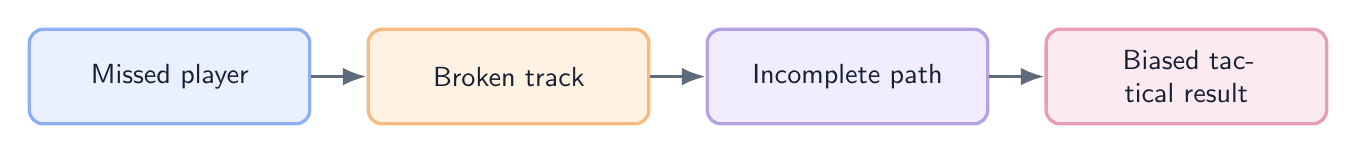
\begin{tikzpicture}[node distance=7mm]
\node[flowblue,text width=3cm] (a) {Missed player};
\node[floworange,text width=3cm,right=of a] (b) {Broken track};
\node[flowpurple,text width=3cm,right=of b] (c) {Incomplete path};
\node[flowpink,text width=3cm,right=of c] (d) {Biased tactical result};
\draw[arrow] (a)--(b);\draw[arrow] (b)--(c);\draw[arrow] (c)--(d);
\end{tikzpicture}
\end{adjustbox}
\end{center}

Include intermediate metrics:

\begin{tabularx}{\textwidth}{>{\bfseries\RaggedRight}p{3cm} Y Y}
\toprule
Module & Suggested metrics & Effect on the final system \\
\midrule
Detection & Precision, recall, mAP and small-object recall & Missing players or balls; false positives.\\
Tracking & IDF1, HOTA, ID switches and coverage & Whether a path belongs to the same person.\\
Geometry & Validation reprojection error and court-position error & Reliability of distance, speed and formations.\\
Team / identity & Accuracy, confusion matrix, switch rate and reject rate & Integrity of team and player statistics.\\
Pose / event & PCK, angle error and release-frame error & Accuracy of motion and event timing.\\
End-to-end & Task completion, analysis error and interpretation time & Practical usefulness.\\
\bottomrule
\end{tabularx}

\section{Baselines and Ablation Studies}

\subsection{Use a Reasonable, Simple Baseline}

For a study of track-level team voting:

\begin{itemize}
  \item Baseline A: Frame-level HSV features and K-means.
  \item Baseline B: Frame-level deep embeddings and a classifier.
  \item Proposed method: Multi-frame embedding averages and confidence-weighted voting.
\end{itemize}

\subsection{Remove Components to Test Their Contribution}

\begin{itemize}
  \item Remove temporal voting to test whether temporal integration causes the improvement.
  \item Remove torso cropping to test the importance of background suppression.
  \item Remove confidence weighting to test whether a simple majority vote is sufficient.
  \item Replace ByteTrack with SORT to assess the contribution of low-score association.
\end{itemize}

\begin{riskBox}
Beating a poorly configured alternative does not establish effectiveness. Baselines must be reasonable, reproducible and fairly tuned. Use the same test split and evaluation procedure for every method.
\end{riskBox}

\section{Data Splits Should Match the Intended Generalization}

\begin{itemize}
  \item Do not randomly divide adjacent frames from the same clip between training and testing.
  \item To test generalization across games, use previously unseen games.
  \item To test new venues, include unseen backgrounds, cameras and lighting.
  \item To test new jerseys, include unseen colors and designs.
  \item Tune all thresholds and parameters on validation data only. Do not revise them after inspecting test results.
\end{itemize}

\section{Apply the Same Sampling Rules to Successes and Failures}

A useful failure taxonomy includes:

\begin{tcbraster}[raster columns=2,raster equal height=rows,raster column skip=7pt,raster row skip=7pt]
\begin{termBox}{Detection failure}
Missed distant balls, spectators mistaken for players, or confusion between a ball and a head.
\end{termBox}
\begin{termBox}{Association failure}
New IDs after occlusion, swapped identities at crossings, or old tracks attached to different players.
\end{termBox}
\begin{termBox}{Geometry failure}
Incorrect calibration points, an outdated $H$ after camera motion, or occluded footpoints.
\end{termBox}
\begin{termBox}{Identity / Team failure}
Similar jerseys, referee contamination, shadow-induced color shifts or invisible numbers.
\end{termBox}
\begin{termBox}{Pose / Event failure}
A ball hiding the wrist, poses assigned to the wrong person, or release rules failing for a shot style.
\end{termBox}
\begin{termBox}{Data / System failure}
Incorrect FPS, unsynchronized timestamps, mixed units or inconsistent field versions.
\end{termBox}
\end{tcbraster}

\section{Presenting the Project}

\begin{center}
\begin{adjustbox}{max width=\linewidth}
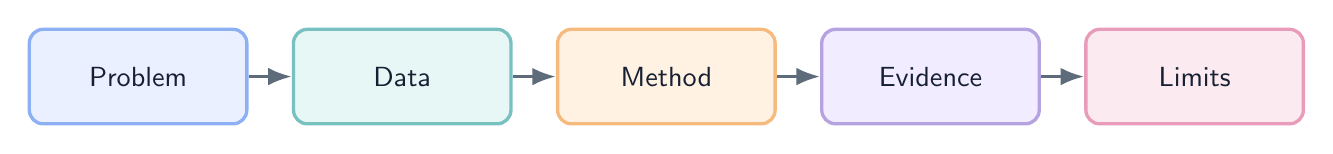
\begin{tikzpicture}[node distance=5.5mm]
\node[flowblue,text width=2.2cm] (p) {Problem};
\node[flowteal,text width=2.2cm,right=of p] (data) {Data};
\node[floworange,text width=2.2cm,right=of data] (method) {Method};
\node[flowpurple,text width=2.2cm,right=of method] (evi) {Evidence};
\node[flowpink,text width=2.2cm,right=of evi] (lim) {Limits};
\draw[arrow] (p)--(data);\draw[arrow] (data)--(method);\draw[arrow] (method)--(evi);\draw[arrow] (evi)--(lim);
\end{tikzpicture}
\end{adjustbox}
\end{center}

\begin{enumerate}
  \item Begin with a concrete use case.
  \item Define inputs, outputs and success criteria.
  \item Use the architecture diagram to explain data flow.
  \item Use tables and curves to compare against baselines.
  \item Show representative cases in the demo; retain formal evaluation separately.
  \item Include failure cases and the next experiment worth conducting.
\end{enumerate}


% ================================================================
% APPENDICES
% ================================================================
\appendix
\titleformat{\chapter}[display]
  {\bfseries\color{Ink}\raggedright\hyphenpenalty=10000}
  {
\begin{tikzpicture}[baseline=(n.base)]\node[fill=Purple,text=white,rounded corners=4pt,inner xsep=9pt,inner ysep=4pt,font=\large\bfseries] (n) {APPENDIX \thechapter};\end{tikzpicture}}
  {8pt}{\Huge}[\vspace{3pt}\color{Line}\titlerule]

\chapter{Glossary}

\begin{longtable}{>{\bfseries\RaggedRight}p{3.6cm} p{4.1cm} p{8cm}}
\toprule
Term & Meaning & Explanation \\
\midrule
\endfirsthead
\toprule
Term & Meaning & Explanation \\
\midrule
\endhead
Pixel & Picture element & The smallest color element in an image; numerical pixel values are the model's initial input.\\
Frame & Still image in a video & One image in a video sequence.\\
FPS & Frames per second & Temporal sampling rate; 30 FPS means 30 frames each second.\\
BBOX & Bounding box & A rectangle approximating an object's location.\\
Keypoint & Defined landmark & A point with a specific meaning, such as a wrist or court-line intersection.\\
Segmentation mask & Pixel-level region & A detailed map of the pixels belonging to an object.\\
Confidence & Model score & A ranking score that need not be a calibrated probability of correctness.\\
IoU & Intersection over union & Overlap area divided by union area for two regions.\\
NMS & Non-maximum suppression & Removes duplicate candidate boxes around the same object.\\
Homography & Planar projective mapping & Maps coordinates from one plane to another.\\
BEV & Bird's-eye view & A shared, approximately top-down representation of the court.\\
Footpoint & Ground-contact estimate & Represents where a player meets the floor.\\
Tracking & Identity over time & Maintains an object's identity across frames.\\
Track ID & Temporary track identifier & An identifier within a video, not a player's name or jersey number.\\
Data association & Observation-to-track matching & Decides which detection should update which track.\\
Kalman filter & Dynamic state estimator & Predicts a state with a motion model, then corrects it using observations.\\
Hungarian algorithm & Optimal assignment & Finds a minimum-total-cost match under one-to-one constraints.\\
ReID & Re-identification & Uses appearance embeddings to help reconnect identity after occlusion.\\
Embedding & Feature vector & Encodes an image crop as a vector whose distance can be compared.\\
Clustering & Unsupervised grouping & Groups observations by feature similarity without class labels.\\
Pose estimation & Body-joint localization & Predicts the positions of body keypoints.\\
Reprojection error & Projection discrepancy & Distance between a projected point and its known reference location.\\
Baseline & Reference method & A reasonable, simple method used for comparison.\\
Ablation & Component-removal study & Removes a component to test its contribution.\\
Domain shift & Change in data conditions & Differences in venue, lighting, cameras or jerseys between training and use.\\
\bottomrule
\end{longtable}

\chapter{Tool Selection Guide}

\begin{tabularx}{\textwidth}{>{\bfseries\RaggedRight}p{3cm} Y Y Y}
\toprule
Need & First option & Strengths & Considerations \\
\midrule
Create a box dataset & Roboflow / CVAT & Full interfaces, collaboration and format conversion & Write annotation rules before labeling at scale.\\
Compare detectors & MMDetection & Broad model library and configurations & Complex configuration; deployment needs preparation.\\
Build a YOLO baseline & Ultralytics & Consistent training, inference and tracking APIs & Pin versions and parameters.\\
Geometry and cameras & OpenCV & Mature, cross-language tools & Successful computation does not validate point selection.\\
Real-time MOT, fixed camera & ByteTrack & Simple, low additional overhead & No appearance cues; long occlusion can change IDs.\\
Moving camera or frequent ID swaps & BoT-SORT & Motion compensation and optional ReID & More parameters and greater cost.\\
Close-up single-person pose & MediaPipe & Lightweight and easy to integrate & Not equivalent to accurate multi-player game pose.\\
Multi-person pose research & MMPose / OpenPose family & Model choice and research flexibility & Small, distant and occluded people remain difficult.\\
Experiment tracking & W\&B / MLflow & Store parameters, curves and artifacts & Define consistent names and dataset versions first.\\
\bottomrule
\end{tabularx}

\chapter{Metric Selection Guide}

\begin{tabularx}{\textwidth}{>{\bfseries\RaggedRight}p{3.3cm} Y Y}
\toprule
Task & Suggested metrics & Failure cases to inspect \\
\midrule
Detection & Precision, recall, AP / mAP, small-object recall & Distant balls, overlapping players and referees mistaken for players.\\
Tracking & IDF1, HOTA, ID switches, coverage & Occlusion, crossings and camera motion.\\
Homography & Validation reprojection error, court-position error & View edges, extrapolated regions and camera displacement.\\
Team classification & Accuracy, macro F1, switch rate, reject rate & White jerseys, shadows, referees and rear views.\\
Pose & PCK, OKS, keypoint AP, angle error & Occlusion, truncation and body rotation.\\
Event timing & Frame MAE, accuracy within a tolerance & Different shot styles and brief ball loss.\\
End-to-end & Task success, final analysis error, user time & Propagation of upstream errors into conclusions.\\
\bottomrule
\end{tabularx}

\chapter{Possible Project Extensions}

\begin{enumerate}
  \item \textbf{Player localization:} Compare BEV errors from box footpoints, ankle keypoints and segmentation-based footpoints.
  \item \textbf{Tracking stability:} Compare SORT, ByteTrack and BoT-SORT IDF1 with fixed and moving cameras.
  \item \textbf{Team recognition:} Compare HSV features, deep embeddings and track-level voting.
  \item \textbf{Possession:} Combine ball-to-player distance, occlusion and temporal states to estimate possession.
  \item \textbf{Shot events:} Combine ball paths, wrist distance and pose signals to estimate the release frame.
  \item \textbf{Spatial analysis:} Use BEV paths to measure spacing, paint occupancy and transition speed.
  \item \textbf{Pose stability:} Compare single-frame pose, moving averages and confidence-weighted temporal filtering using joint jitter and angle error.
  \item \textbf{Uncertainty:} Report position intervals and event confidence, and allow the system to abstain when evidence is insufficient.
\end{enumerate}

\renewcommand{\bibname}{References and Further Reading}
\small
\begin{thebibliography}{99}
\phantomsection\addcontentsline{toc}{chapter}{References and Further Reading}
\bibitem{ransac} Martin A. Fischler and Robert C. Bolles. Random Sample Consensus: A Paradigm for Model Fitting with Applications to Image Analysis and Automated Cartography. \textit{Communications of the ACM}, 1981.
\bibitem{hog} Navneet Dalal and Bill Triggs. Histograms of Oriented Gradients for Human Detection. CVPR, 2005.
\bibitem{rcnn} Ross Girshick et al. Rich Feature Hierarchies for Accurate Object Detection and Semantic Segmentation. CVPR, 2014.
\bibitem{fasterrcnn} Shaoqing Ren et al. Faster R-CNN: Towards Real-Time Object Detection with Region Proposal Networks. NeurIPS, 2015.
\bibitem{yolo} Joseph Redmon et al. You Only Look Once: Unified, Real-Time Object Detection. CVPR, 2016.
\bibitem{detr} Nicolas Carion et al. End-to-End Object Detection with Transformers. ECCV, 2020.
\bibitem{sort} Alex Bewley et al. Simple Online and Realtime Tracking. ICIP, 2016.
\bibitem{deepsort} Nicolai Wojke, Alex Bewley, and Dietrich Paulus. Simple Online and Realtime Tracking with a Deep Association Metric. ICIP, 2017.
\bibitem{bytetrack} Yifu Zhang et al. ByteTrack: Multi-Object Tracking by Associating Every Detection Box. ECCV, 2022.
\bibitem{botsort} Nir Aharon, Roy Orfaig, and Ben-Zion Bobrovsky. BoT-SORT: Robust Associations Multi-Pedestrian Tracking. arXiv:2206.14651, 2022.
\bibitem{hota} Jonathon Luiten et al. HOTA: A Higher Order Metric for Evaluating Multi-Object Tracking. International Journal of Computer Vision, 2021.
\bibitem{openpose} Zhe Cao et al. OpenPose: Realtime Multi-Person 2D Pose Estimation Using Part Affinity Fields. IEEE TPAMI, 2021.
\bibitem{hrnet} Ke Sun et al. Deep High-Resolution Representation Learning for Human Pose Estimation. CVPR, 2019.
\bibitem{blazepose} Valentin Bazarevsky et al. BlazePose: On-device Real-time Body Pose Tracking. arXiv:2006.10204, 2020.
\bibitem{integralpose} Xiao Sun et al. Integral Human Pose Regression. ECCV, 2018.
\bibitem{simcc} Yanjie Li et al. SimCC: a Simple Coordinate Classification Perspective for Human Pose Estimation. ECCV, 2022.
\bibitem{vitpose} Yufei Xu et al. ViTPose: Simple Vision Transformer Baselines for Human Pose Estimation. NeurIPS, 2022.
\bibitem{rtmpose} Tao Jiang et al. RTMPose: Real-Time Multi-Person Pose Estimation Based on MMPose. arXiv:2303.07399, 2023.
\bibitem{opencv} OpenCV Documentation. Basic Concepts of the Homography Explained with Code. \url{https://docs.opencv.org/4.x/d9/dab/tutorial_homography.html}
\bibitem{ultralytics} Ultralytics Documentation. Multi-Object Tracking with BoT-SORT and ByteTrack. \url{https://docs.ultralytics.com/modes/track/}
\bibitem{roboflow} Roboflow Documentation. Annotation Tools and Project Types. \url{https://docs.roboflow.com/annotate/annotation-tools}
\end{thebibliography}
\normalsize

\begin{heroBox}
\textbf{Closing note:}\quad
This handout provides a framework for further analysis. Define the question and output before choosing data and methods. Retain intermediate results and evaluate each stage. Support conclusions with evidence and state the system's limits clearly.
\end{heroBox}

\end{document}
